% Options for packages loaded elsewhere
\PassOptionsToPackage{unicode}{hyperref}
\PassOptionsToPackage{hyphens}{url}
%
\documentclass[
]{article}
\usepackage{lmodern}
\usepackage{amssymb,amsmath}
\usepackage{ifxetex,ifluatex}
\ifnum 0\ifxetex 1\fi\ifluatex 1\fi=0 % if pdftex
  \usepackage[T1]{fontenc}
  \usepackage[utf8]{inputenc}
  \usepackage{textcomp} % provide euro and other symbols
\else % if luatex or xetex
  \usepackage{unicode-math}
  \defaultfontfeatures{Scale=MatchLowercase}
  \defaultfontfeatures[\rmfamily]{Ligatures=TeX,Scale=1}
\fi
% Use upquote if available, for straight quotes in verbatim environments
\IfFileExists{upquote.sty}{\usepackage{upquote}}{}
\IfFileExists{microtype.sty}{% use microtype if available
  \usepackage[]{microtype}
  \UseMicrotypeSet[protrusion]{basicmath} % disable protrusion for tt fonts
}{}
\makeatletter
\@ifundefined{KOMAClassName}{% if non-KOMA class
  \IfFileExists{parskip.sty}{%
    \usepackage{parskip}
  }{% else
    \setlength{\parindent}{0pt}
    \setlength{\parskip}{6pt plus 2pt minus 1pt}}
}{% if KOMA class
  \KOMAoptions{parskip=half}}
\makeatother
\usepackage{xcolor}
\IfFileExists{xurl.sty}{\usepackage{xurl}}{} % add URL line breaks if available
\IfFileExists{bookmark.sty}{\usepackage{bookmark}}{\usepackage{hyperref}}
\hypersetup{
  pdftitle={Supplementary Information},
  hidelinks,
  pdfcreator={LaTeX via pandoc}}
\urlstyle{same} % disable monospaced font for URLs
\usepackage[margin=1in]{geometry}
\usepackage{graphicx}
\makeatletter
\def\maxwidth{\ifdim\Gin@nat@width>\linewidth\linewidth\else\Gin@nat@width\fi}
\def\maxheight{\ifdim\Gin@nat@height>\textheight\textheight\else\Gin@nat@height\fi}
\makeatother
% Scale images if necessary, so that they will not overflow the page
% margins by default, and it is still possible to overwrite the defaults
% using explicit options in \includegraphics[width, height, ...]{}
\setkeys{Gin}{width=\maxwidth,height=\maxheight,keepaspectratio}
% Set default figure placement to htbp
\makeatletter
\def\fps@figure{htbp}
\makeatother
\setlength{\emergencystretch}{3em} % prevent overfull lines
\providecommand{\tightlist}{%
  \setlength{\itemsep}{0pt}\setlength{\parskip}{0pt}}
\setcounter{secnumdepth}{-\maxdimen} % remove section numbering
\usepackage{float} \usepackage{caption} \captionsetup[table]{font=footnotesize} \captionsetup[figure]{font=footnotesize} \captionsetup[figure]{labelformat=empty} \captionsetup[table]{labelformat=empty} \usepackage{pdflscape} \newcommand{\blandscape}{\begin{landscape}} \newcommand{\elandscape}{\end{landscape}}
\usepackage{booktabs}
\usepackage{longtable}
\usepackage{array}
\usepackage{multirow}
\usepackage{wrapfig}
\usepackage{float}
\usepackage{colortbl}
\usepackage{pdflscape}
\usepackage{tabu}
\usepackage{threeparttable}
\usepackage{threeparttablex}
\usepackage[normalem]{ulem}
\usepackage{makecell}
\usepackage{xcolor}
\ifluatex
  \usepackage{selnolig}  % disable illegal ligatures
\fi
\newlength{\cslhangindent}
\setlength{\cslhangindent}{1.5em}
\newenvironment{cslreferences}%
  {\setlength{\parindent}{0pt}%
  \everypar{\setlength{\hangindent}{\cslhangindent}}\ignorespaces}%
  {\par}

\title{Supplementary Information}
\author{}
\date{\vspace{-2.5em}}

\begin{document}
\maketitle

{
\setcounter{tocdepth}{3}
\tableofcontents
}
\newpage

\hypertarget{appendix-s1.-methods-for-reconstruction-of-dbh}{%
\subsection{\texorpdfstring{Appendix S1. Methods for reconstruction of
\(DBH\)}{Appendix S1. Methods for reconstruction of DBH}}\label{appendix-s1.-methods-for-reconstruction-of-dbh}}

\emph{This is still rough/ mostly notes.}

For each core, \(DBH\) can be reconstructed outside-in (based on recent
\(DBH\), subtracting growth recorded in tree rings) or inside-out
(summing \(\Delta r\) from the inside out). We generally gave precedence
to the outside-in approach. Specifically, when \(DBH\) was taken at the
time of coring,\\
At some of our sites where DBH was not taken at the time of coring
(\emph{SCBI},), DBH measurements taken before or slightly after the time
of coring could be used. (see
\href{https://github.com/EcoClimLab/ForestGEO_dendro/issues/19}{issue
\#19 in ForestGEO\_dendro}) If before, \ldots{} If after\ldots{} For all
outside-in reconstructions, if a negative \(DBH\) was predicted\ldots{}

When there were more than one cores for a tree, the \(DBH\)
reconstructions from each core were averaged to produce a single
estimate of the tree's \(DBH\) through time. When the start or end dates
of the records from the cores differed, we extrapolated growth of the
shorter core to match the years covered by the longer core.
Specifically, to fill in years at the more recent end, we assumed that
the average growth rate of the ten years prior to the missing records
applied to the missing years. To fill in years at the beginning of the
tree's lifespan, we likewise assumed that the ten years adjacent to the
missing record applied to the missing years; however, if this yielded a
negative \(DBH\) estimate for the earliest year in the reconstruction,
we divided the existing minimum \(DBH\) by number of years missing and
applied that value to each year. We note that these reconstructed growth
records were used only for the reconstruction of \(DBH\) and were not
included as response variables in any of our analyses.

In either case we need bark thickness--ideally allometries describing
the relationship between DBH and bark thickness (Table S4). This is
especially critical for thick-barked species. When bark thickness data
were available, we generated allometries
(\href{https://github.com/EcoClimLab/ForestGEO_dendro/issues/8}{issue
\#8 in ForestGEO\_dendro})\ldots{} lognormal model with intercept forced
to zero:
\texttt{lm(bark\_depth.mm\ \textasciitilde{}\ -1\ +\ log(dbh\_no\_bark.cm+1):bark\_species,\ data\ =\ bark)}.
When bark thickness data were not available, we used published bark
allometries from other sources (Table S4)

\newpage

\hypertarget{appendix-s2.-methods-for-comparing-climwin-results-with-traditional-methods}{%
\subsection{Appendix S2. Methods for comparing climwin results with
traditional
methods}\label{appendix-s2.-methods-for-comparing-climwin-results-with-traditional-methods}}

\emph{(\href{https://github.com/EcoClimLab/ForestGEO-climate-sensitivity/issues/35}{ISSUE
\#35 in ForestGEO-climate-sensitivity})}

To verify that our methods gave similar results to traditional methods,
we conducted qualitative comparisons of our results to previous studies
based on the same cores (Table \textbf{S5}). We also conducted a formal
comparison using identical tree-ring and climate data for four
well-studied species: PSME (Cedar Breaks, Utah), ABAL (Zofin), PIMA
(Scotty Creek), and LITU (SCBI) (Fig. \textbf{S1}). We compared results
from an analysis using conventional methods, as detailed below, to an
analysis using our method as described in the Methods section, but with
the \emph{climwin} climate variable selection process limited to just
the species of interest (as opposed to all species at the site), climate
variables considered individually rather than additively, and with start
date adjusted to match the conventional method.

The ring-width series from each core was standardized via ARSTAN using a
2/3rds \(n\) spline, where \(n\) is the number of years in the series
(\emph{Cook, 1985; Cook \& Kairiukstis, 1990- citations in Helcoski}).
\emph{(The following italic text is plagarized from Helcoski and needs
to be reworded:)} \emph{The influence of outliers in all series was
reduced using the adaptive power transformation, which also stabilises
the variance over time (Cook \& Peters, 1997). Next, each series was
stabilised using either the average correlation between raw ring-width
series (rbar) method or a 1/ 3rds spline method to adjust changes in
variance as series replication decreased towards the earlier portion of
each chronology (Jones et al., 1997). The 1/3rds spline method was
chosen when replication in the inner portion of each chronology (c.~the
inner 30--50 yr of each record depending on full chronology length)
dropped below three trees. Once that step was complete, a robust
biweight mean chronology for each species was calculated from the
ring-width indices (Cook, 1985). We chose to use residual chronologies
because the autoregressive standardisation process in creating them
removes much of the tree-level autocorrelation in growth and these
chronologies would most likely contain the most conservative information
on drivers of interannual growth (Cook, 1985).}

Following Helcoski et al. (2019), we defined chronology start dates
according to the subsample signal strength (SSS), using a cutoff of SSS
= 0.80 (or 80\% of the population signal). Thus, for this analysis only,
we defined chronology start dates as the year the SSS exceeded 0.80 or
two years after the start of the climate record, whichever came later.
SSS exceeded 0.80 well before the start of the 1901 start of climate
records for PSME (1800s), ABAL (1700), and PIMA (1850s). For LITU , SSS
reached 0.8 with 11 trees in 1919, which we used as the start date for
this series. We note that these start date criteria differ from those
used in the main analysis (Table S3), which had earlier start dates
because the analysis was not constrained by a need to represent the full
population signal. End dates were defined as the last full year prior to
sampling (Table S3).

\newpage

\hypertarget{appendix-s3.-dealing-with-rapidly-changing-climate-and-tree-growth}{%
\subsection{Appendix S3. Dealing with rapidly changing climate and tree
growth}\label{appendix-s3.-dealing-with-rapidly-changing-climate-and-tree-growth}}

\href{https://github.com/EcoClimLab/ForestGEO-climate-sensitivity/issues/25}{ISSUE
\#25 in ForestGEO-climate-sensitivity}

Our analysis included two sites where climate change has had pronounced
effects on tree growth: Scotty Creek, NW Territories, Canada (SC) and
Little Tesuque, New Mexico, USA (LT). At SC, {[}temperatures have
increased by X \(^\circ\) over X years{]}\ldots, resulting in negative
growth trends in basal area index (\(BAI\)) starting around 1950 and
significant growth declines since 1970 in 56\% of trees (Sniderhan \&
Baltzer, 2016). At LT, \emph{(drought has increased dramatically)},
resulting in many missing rings in recent years.

\emph{This is in process. We will try and compare 3 methods: (1) our
standard approach, (2) detrending the climate variables (\#53), (3)
applying the climwin step only for older records--before the most rapid
climate change. We will work with SC and LT researchers to determine
which makes most sense, and use that as the main approach for these
sites.}

\newpage

\hypertarget{table-s1.-site-details}{%
\subsection{Table S1. Site Details}\label{table-s1.-site-details}}

\begin{table}[!h]
\centering
\resizebox{\linewidth}{!}{
\begin{tabular}{l>{\raggedright\arraybackslash}p{3cm}rr>{\raggedright\arraybackslash}p{2cm}>{\raggedright\arraybackslash}p{2cm}>{\raggedright\arraybackslash}p{1.5cm}llll}
\toprule
site code & site name & latitude & longitude & elevation (m.a.s.l.) & cores within ForestGEO plot? & canopy positions & tree statuses & date range & dormant season & months in climwin\\
\midrule
BCI & Barro Colorado Island & 9.15430 & -79.8461 & 120-160 & no & canopy & live, dead & 1931-2014 & Nov-Apr & pOct-cDec\\
HKK & Huai Kha Khaeng & 15.63240 & 99.2170 & 549-638 & no & all & live & 1903-2011 & Nov-Apr & pOct-cDec\\
LT & Little Tesuque & 35.73838 & -105.8382 & 2682 & n.a. & all & live & 1903-2018 &  & pMay-cAug\\
CB & Utah Forest Dynamics Plot & 37.66150 & -112.8525 & 3020-3169 & yes &  & live & 1903-2007 &  & pMay-cAug\\
SCBI & Smithsonian Conservation Biology Institute & 38.89350 & -78.1454 & 273-338 & yes & all & live, dead & 1903-2017 & Oct-Apr & pMay-cAug\\
\addlinespace
LDW & Lilly Dickey Woods & 39.23590 & -86.2181 & 230-303 &  & canopy & live, dead & 1903-2019 &  & pMay-cAug\\
HF & Harvard Forest & 42.53880 & -72.1755 & 340-368 & yes & all & live, dead & 1903-2014 &  & pMay-cAug\\
NE & Niobrara/Halsey & 42.78000 & -100.0210 & 644-702 & some & canopy & live &  & Oct-Apr & pMay-cAug\\
ZOF & $\v{Z}$of$\'{i}$n Forest Dynamics Plot & 48.66380 & 14.7073 & 736-829 & some & all & live, dead & 1903-2013 & Oct-Mar & pMay-cAug\\
SC & Scotty Creek & 61.30000 & -121.3000 & 258-274 & no & all & live, dead & 1903-2013 &  & pMay-cAug\\
\bottomrule
\end{tabular}}
\end{table}

\newpage

\hypertarget{table-s2.-species-analyzed-their-characteristics-and-bark-allometries-applied}{%
\subsection{Table S2. Species analyzed, their characteristics, and bark
allometries
applied}\label{table-s2.-species-analyzed-their-characteristics-and-bark-allometries-applied}}

\emph{(\href{https://github.com/EcoClimLab/ForestGEO-climate-sensitivity/issues/72}{ISSUE
\#72 in ForestGEO-climate-sensitivity})}

\emph{NOTE: bark.allometry field is not yet right-- we will have just
one latin name per site, corresponding to allometries in Table S4. But
it does give correct info for what is currently applied. We also intend
to find and apply more allometries.}

\begin{table}[!h]
\centering
\resizebox{\linewidth}{!}{
\begin{tabular}{lllllll>{\raggedright\arraybackslash}p{5cm}}
\toprule
\textbf{species code} & \textbf{family} & \textbf{latin name} & \textbf{sites sampled} & \textbf{leaf type} & \textbf{leaf phenology} & \textbf{light requirements} & \textbf{bark allometry}\\
\midrule
ABAL & Pinaceae & Abies alba & ZOF & needleleaf & evergreen & shade-tolerant & neglected in Zofin\\
\addlinespace
ABBI & Pinaceae & Abies bifolia & CB & needleleaf & evergreen &  & neglected in CedarBreaks\\
\addlinespace
ACRU & Sapindaceae & Acer rubrum & HF & broadleaf & deciduous (cold) &  & acru in HarvardForest\\
\addlinespace
ACSA & Sapindaceae & Acer saccharum & LDW & broadleaf & deciduous (cold) &  & acru in LillyDickey, acru in LillyDickey\\
\addlinespace
AFXY & Fabaceae & Afzelia xylocarpa & HKK & broadleaf & deciduous (drought) &  & neglected in HKK\\
\addlinespace
BEAL & Betulaceae & Betula alleghaniensis & HF & broadleaf & deciduous (cold) &  & Betula alleghaniensis in HarvardForest\\
\addlinespace
BEPA & Betulaceae & Betula papyrifera & NE & broadleaf & deciduous (cold) &  & Betula papyrifera in Nebraska\\
\addlinespace
CACO & Juglandaceae & Carya cordiformis & SCBI & broadleaf & deciduous (cold) &  & caco in SCBI\\
\addlinespace
CAGL & Juglandaceae & Carya glabra & SCBI & broadleaf & deciduous (cold) &  & cagl in SCBI\\
\addlinespace
CAOV & Juglandaceae & Carya ovata & LDW & broadleaf & deciduous (cold) &  & cagl in LillyDickey\\
\addlinespace
CAOVL & Juglandaceae & Carya ovalis & SCBI & broadleaf & deciduous (cold) &  & caovl in SCBI\\
\addlinespace
CATO & Juglandaceae & Carya tomentosa & SCBI & broadleaf & deciduous (cold) &  & cato in SCBI\\
\addlinespace
CHTA & Meliaceae & Chukrasia tabularis & HKK & broadleaf & brevi-deciduous (drought) &  & neglected in HKK\\
\addlinespace
FAGR & Fagaceae & Fagus grandifolia & HF, SCBI & broadleaf & deciduous (cold) &  & neglected in HarvardForest, neglected in LillyDickey, neglected in SCBI\\
\addlinespace
FASY & Fagaceae & Fagus sylvatica & ZOF & broadleaf & deciduous (cold) & shade-tolerant & neglected in Zofin\\
\addlinespace
FRAM & Oleaceae & Fraxinus americana & LDW, SCBI & broadleaf & deciduous (cold) &  & Fraxinus ssp. in LillyDickey, fram in SCBI\\
\addlinespace
FRNI & Oleaceae & Fraxinus nigra & SCBI & broadleaf & deciduous (cold) &  & fram in SCBI\\
\addlinespace
JACO & Bignoniaceae & Jacaranada copaia & BCI & broadleaf & deciduous (drought) & light-demanding & JCO in BCI\\
\addlinespace
JUNI & Juglandaceae & Juglans nigra & SCBI & broadleaf & deciduous (cold) &  & juni in SCBI\\
\addlinespace
JUVI & Cupressaceae & Juniperus virginiana & NE &  &  &  & neglected in Nebraska\\
\addlinespace
LITU & Magnoliaceae & Liriodendron tulipifera & LDW, SCBI & broadleaf & deciduous (cold) &  & litu in LillyDickey, litu in LillyDickey, litu in SCBI\\
\addlinespace
MEAZ & Meliaceae & Melia azedarach & HKK & broadleaf & deciduous (drought) & light-demanding & neglected in HKK\\
\addlinespace
PIAB & Pinaceae & Picea abies & HF & needleleaf & evergreen & intermediate & neglected in HarvardForest, neglected in Zofin\\
\addlinespace
PIEN & Pinaceae & Picea engelmannii & CB & needleleaf & evergreen &  & Picea engelmannii in CedarBreaks\\
\addlinespace
PIFL & Pinaceae & Pinus flexilis & CB & needleleaf & evergreen &  & Pinus monticola in CedarBreaks\\
\addlinespace
PILO & Pinaceae & Pinus longaeva & CB & needleleaf & evergreen &  & neglected in CedarBreaks\\
\addlinespace
PIMA & Pinaceae & Picea mariana & SC & needleleaf & evergreen &  & PIMA in ScottyCreek\\
\addlinespace
PIPO & Pinaceae & Pinus ponderosa & NE, LT & needleleaf & evergreen &  & Pinus jeffreyi in Little Tesuque, Pinus jeffreyi in Nebraska\\
\addlinespace
PIPU & Pinaceae & Picea pungens & CB & needleleaf & evergreen &  & neglected in CedarBreaks\\
\addlinespace
PIST & Pinaceae & Pinus strobus & HF, SCBI & needleleaf & evergreen &  & Pinus strobus in HarvardForest, pist in SCBI\\
\addlinespace
PIST2 & Pinaceae & Pinus strobiformis & LT & needleleaf & evergreen &  & Pinus monticola in Little Tesuque\\
\addlinespace
POTR & Salicaceae & Populus tremuloides & CB & broadleaf & deciduous (cold) &  & Populus tremuloides in CedarBreaks\\
\addlinespace
PSME & Pinaceae & Pseudotsuga menziesii & CB & needleleaf & evergreen &  & Pseudotsuga menziesii in CedarBreaks\\
\addlinespace
QUAL & Fagaceae & Quercus alba & LDW, SCBI & broadleaf & deciduous (cold) &  & qual in LillyDickey, qual in SCBI\\
\addlinespace
QUMO & Fagaceae & Quercus montana & LDW, SCBI & broadleaf & deciduous (cold) &  & qupr in LillyDickey, qupr in SCBI\\
\addlinespace
QURU & Fagaceae & Quercus rubra & HF, LDW, SCBI & broadleaf & deciduous (cold) &  & quru in HarvardForest, Quercus rubra in LillyDickey, quru in SCBI\\
\addlinespace
QUVE & Fagaceae & Quercus velutina & LDW, SCBI & broadleaf & deciduous (cold) &  & quve in LillyDickey, quve in SCBI\\
\addlinespace
TEPA & Burseraceae & Tetragastris panamensis & BCI & broadleaf & evergreen & shade-tolerant & TPA in BCI\\
\addlinespace
TOCI & Meliaceae & Toona ciliata & HKK & broadleaf & deciduous (drought) &  & neglected in HKK\\
\addlinespace
TRTU & Meliaceae & Trichilia tuberculata & BCI & broadleaf & evergreen & shade-tolerant & TTU in BCI\\
\addlinespace
TSCA & Pinaceae & Tsuga canadensis & HF & needleleaf & evergreen &  & Tsuga canadensis in HarvardForest\\
\bottomrule
\end{tabular}}
\end{table}

*Bark allometry field indicates the species and site sampled to
construct the bark allometry. When neither raw data nor an allometric
equation for the study species was available, we selected the most
appropriate equation that could be located for similar species.
Equations are given in Table S4.

\newpage

\hypertarget{table-s3.-sampling-details-for-species-by-site}{%
\subsection{Table S3. Sampling details for species by
site}\label{table-s3.-sampling-details-for-species-by-site}}

\emph{(\href{https://github.com/EcoClimLab/ForestGEO-climate-sensitivity/issues/73}{ISSUE
\#73 in ForestGEO-climate-sensitivity})}

\begin{table}[!h]
\centering
\resizebox{\linewidth}{!}{
\begin{tabular}{llrrrrlll}
\toprule
\textbf{site} & \textbf{species code} & \textbf{n trees all} & \textbf{n cores all} & \textbf{n trees dbh} & \textbf{n cores dbh} & \textbf{dbh range sampled} & \textbf{dbh range reconstructed*} & \textbf{date range}\\
\midrule
BCI & JACO & 12 & 18 & 11 & 17 & 30.2-63.5 & 2.6-56.4 & 1931-2014\\
\addlinespace
BCI & TEPA & 18 & 29 & 17 & 26 & 22.1-59.5 & 2.7-49.4 & 1931-2014\\
\addlinespace
BCI & TRTU & 23 & 37 & 20 & 31 & 20.7-43.6 & 4.8-41.5 & 1931-2014\\
\addlinespace
CB & ABBI & 22 & 41 & 20 & 37 & 13.9-54.2 & 0.9-46.4 & 1903-2000\\
\addlinespace
CB & PIEN & 12 & 21 & 10 & 15 & 14-54.9 & 0.9-33.1 & 1903-2000\\
\addlinespace
CB & PIFL & 13 & 22 & 12 & 21 & 17.6-64.1 & 1.5-47.5 & 1903-1998\\
\addlinespace
CB & PILO & 11 & 16 & 8 & 12 & 45.8-121.6 & 35.4-118.5 & 1903-1999\\
\addlinespace
CB & PIPU & 15 & 28 & 15 & 28 & 22.4-50.8 & 9.5-48.4 & 1903-2000\\
\addlinespace
CB & POTR & 17 & 27 & 17 & 26 & 23.6-47.6 & 4.3-35.4 & 1903-2000\\
\addlinespace
CB & PSME & 11 & 20 & 10 & 18 & 20.7-64.2 & 0.5-41.5 & 1903-1999\\
\addlinespace
HF & ACRU & 18 & 59 & 18 & 59 & 10.1-22.1 & 0.9-20.4 & 1903-2013\\
\addlinespace
HF & BEAL & 13 & 44 & 13 & 44 & 10.2-37.9 & 0-17.2 & 1904-2013\\
\addlinespace
HF & QURU & 74 & 180 & 73 & 177 & 19.5-53 & 1.1-48.3 & 1903-2014\\
\addlinespace
HF & TSCA & 32 & 83 & 32 & 71 & 10.6-37 & 0-28.4 & 1923-2014\\
\addlinespace
HKK & AFXY & 39 & 127 & 39 & 127 & 20.1-98.7 & 0.1-81.4 & 1903-2011\\
\addlinespace
HKK & CHTA & 28 & 70 & 28 & 70 & 16-64.6 & 0.2-59.5 & 1904-2010\\
\addlinespace
HKK & MEAZ & 46 & 130 & 46 & 130 & 25.6-98.1 & 3.8-80.3 & 1914-2011\\
\addlinespace
HKK & TOCI & 45 & 143 & 45 & 143 & 16.6-116.4 & 1.7-80.5 & 1903-2011\\
\addlinespace
LDW & ACSA & 35 & 66 & 34 & 64 & 9-64.6 & 0-52.4 & 1903-2019\\
\addlinespace
LDW & CAOV & 9 & 18 & 8 & 15 & NA-NA & 1.4-37.4 & 1903-2013\\
\addlinespace
LDW & LITU & 15 & 28 & 14 & 25 & NA-NA & 1.2-69.4 & 1903-2019\\
\addlinespace
LDW & QUAL & 10 & 20 & NA & NA & NA & NA & 1903-2013\\
\addlinespace
LDW & QUMO & 10 & 20 & 8 & 16 & NA-NA & 1.1-52.4 & 1903-2013\\
\addlinespace
LDW & QUVE & 9 & 18 & NA & NA & NA & NA & 1903-2013\\
\addlinespace
NE & BEPA & 28 & 84 & 28 & 84 & NA-NA & 0-25.5 & 1903-1995\\
\addlinespace
NE & JUVI & 29 & 60 & 29 & 60 & 16.6-21.5 & 0.3-18.4 & 1938-1994\\
\addlinespace
NE & PIPO & 71 & 134 & 70 & 129 & 19.3-64 & 0-41.1 & 1934-1994\\
\addlinespace
LT & PIPO & 10 & 20 & 10 & 20 & 23.2-52.8 & 14.4-48.4 & 1903-2018\\
\addlinespace
LT & PIST2 & 7 & 14 & 7 & 14 & 25.7-39.8 & 3.9-34.5 & 1903-2018\\
\addlinespace
SCBI & CACO & 15 & 15 & 14 & 14 & 10.62-38.52 & 1.7-32.2 & 1903-2015\\
\addlinespace
SCBI & CAGL & 39 & 39 & 36 & 36 & 10.28-52.31 & 1.6-49.3 & 1903-2015\\
\addlinespace
SCBI & CAOVL & 25 & 25 & 24 & 24 & 15.11-60.32 & 2.6-47.2 & 1903-2015\\
\addlinespace
SCBI & CATO & 15 & 15 & 14 & 14 & 12.86-35.95 & 3.7-28.4 & 1903-2015\\
\addlinespace
SCBI & FAGR & 76 & 76 & 74 & 74 & 10.05-41.02 & 0.1-41.2 & 1920-2009\\
\addlinespace
SCBI & FRAM & 66 & 66 & 61 & 61 & 8.11-94.73 & 0.1-84.4 & 1903-2016\\
\addlinespace
SCBI & FRNI & 12 & 12 & 12 & 12 & 11.04-39.2 & 0.5-27.3 & 1903-1996\\
\addlinespace
SCBI & JUNI & 30 & 30 & 28 & 28 & 20.4-76.19 & 5.6-59.5 & 1903-2010\\
\addlinespace
SCBI & LITU & 106 & 106 & 104 & 104 & 10-91.42 & 0.1-81.1 & 1903-2010\\
\addlinespace
SCBI & PIST & 36 & 36 & 36 & 36 & 13.92-50.96 & 1.6-45.2 & 1931-2010\\
\addlinespace
SCBI & QUAL & 66 & 66 & 66 & 66 & 11.4-76.73 & 0.3-70.4 & 1903-2009\\
\addlinespace
SCBI & QUMO & 67 & 67 & 67 & 67 & 10.22-84.59 & 0.3-69.5 & 1903-2017\\
\addlinespace
SCBI & QURU & 70 & 70 & 70 & 70 & 11.07-87.65 & 2.5-79.2 & 1903-2016\\
\addlinespace
SCBI & QUVE & 81 & 81 & 81 & 81 & 16.02-82.33 & 0.5-78.4 & 1903-2009\\
\addlinespace
SC & PIMA & 442 & 442 & 101 & 101 & 7-14.9 & 0.5-12.5 & 1903-2013\\
\addlinespace
ZOF & ABAL & 55 & 55 & 50 & 50 & 41-121 & 21.3-108.5 & 1903-2011\\
\addlinespace
ZOF & FASY & 1369 & 1369 & 1358 & 1358 & NA-NA & 0.1-115.3 & 1903-2013\\
\addlinespace
ZOF & PCAB & 644 & 644 & 599 & 599 & NA-NA & 0.5-126.4 & 1903-2011\\
\bottomrule
\end{tabular}}
\end{table}

*Maximum reconstructed \(DBH\)'s analyzed are less than maximum sampled
\(DBH\)'s because we discard size ranges with \textless{} 3 conspecific
trees.

\newpage

\hypertarget{table-s4.-allometric-equations-for-bark-thickness}{%
\subsection{Table S4. Allometric equations for bark
thickness}\label{table-s4.-allometric-equations-for-bark-thickness}}

\begin{table}[!h]
\centering
\resizebox{\linewidth}{!}{
\begin{tabular}{>{}llrl>{\raggedright\arraybackslash}p{3cm}>{\raggedright\arraybackslash}p{6cm}}
\toprule
\textbf{species} & \textbf{equation} & \textbf{n} & \textbf{DBH.range.cm} & \textbf{site} & \textbf{source}\\
\midrule
\em{Acer rubrum} & $bark.mm = 0.619 * log(dbh.cm + 1)$ & 10 & 8.2-39.6 & SCBI & Anderson-Teixeira et al. (2015)\\
\addlinespace
\em{Betula alleghaniensis} & $bark.mm = (0.15 + 0.03 * dbh.cm)/2$ & NA &  & North America average of its range & Miles, Patrick D.; Smith, W. Brad. 2009.\\
\addlinespace
\em{Betula papyrifera} & $bark.mm = (0.13 + 0.05 * dbh.cm)/2$ & NA &  & North America average of its range & Miles, Patrick D.; Smith, W. Brad. 2009.\\
\addlinespace
\em{Carya cordiformis} & $bark.mm = 0.793 * log(dbh.cm + 1)$ & 9 & 5.9-68.2 & SCBI & Anderson-Teixeira et al. (2015)\\
\addlinespace
\em{Carya ovalis} & $bark.mm = 1.531 * log(dbh.cm + 1)$ & 8 & 6.4-63.1 & SCBI & Anderson-Teixeira et al. (2015)\\
\addlinespace
\em{Carya ovata} & $bark.mm = 1.035 * log(dbh.cm + 1)$ & 8 & 19.1-78 & SCBI & Anderson-Teixeira et al. (2015)\\
\addlinespace
\em{Carya tomentosa} & $bark.mm = 1.105 * log(dbh.cm + 1)$ & 8 & 5-57.3 & SCBI & Anderson-Teixeira et al. (2015)\\
\addlinespace
\em{Fraxinus americana} & $bark.mm = 2.223 * log(dbh.cm + 1)$ & 9 & 6.1-94.2 & SCBI & Anderson-Teixeira et al. (2015)\\
\addlinespace
\em{Fraxinus americana} & $bark.mm = (0.38 + 0.05 * dbh.cm)/2$ & NA &  & North America average of its range & Miles, Patrick D.; Smith, W. Brad. 2009.\\
\addlinespace
\em{Jacaranada copaia} & $bark.mm = 2.993 * log(dbh.cm + 1)$ & 5 & 45.6-75 & Panama & Raquel Alfaro-S$\acute{a}$nchez (unpublished data)\\
\addlinespace
\em{Juglans nigra} & $bark.mm = 2.107 * log(dbh.cm + 1)$ & 9 & 13.6-85.4 & SCBI & Anderson-Teixeira et al. (2015)\\
\addlinespace
\em{Liriodendron tulipifera} & $bark.mm = 1.637 * log(dbh.cm + 1)$ & 9 & 27.5-136.5 & SCBI & Anderson-Teixeira et al. (2015)\\
\addlinespace
\em{Picea engelmannii} & $bark.mm = (0.15 + 0.04 * dbh.cm)/2$ & NA &  & North America average of its range & Miles, Patrick D.; Smith, W. Brad. 2009.\\
\addlinespace
\em{Picea mariana} & $bark.mm = 3.726 * log(dbh.cm + 1)$ & 12 & 6.9-7.9 & Scotty Creek & Anastasia Sniderhan and Jennifer Baltzer (unpublished data)\\
\addlinespace
\em{Pinus flexilis} & $bark.mm = (1.299*\sqrt(dbh.cm)^{0.609})^{2}$ & 29 & ~10-130 & California (3 montane sites) & Zeibig-Kichas et al. (2016)\\
\addlinespace
\em{Pinus ponderosa} & $bark.mm = (1.298*\sqrt(dbh.cm)^{0.802})^{2}$ & 81 & ~5-160 & California (4 montane sites) & Zeibig-Kichas et al. (2016)\\
\addlinespace
\em{Pinus strobus} & $bark.mm = 1.568 * log(dbh.cm + 1)$ & 1 & 28.4-28.4 & Illinois & Miles and Smith (2009)\\
\addlinespace
\em{Pinus strobus} & $bark.mm = (0.02 + 0.10 * dbh.cm)/2$ & NA &  & North America average of its range & Miles, Patrick D.; Smith, W. Brad. \vphantom{1} 2009.\\
\addlinespace
\em{Pinus strobus} & $bark.mm = (0.02 + 0.10 * dbh.cm)/2$ & NA &  & North America average of its range & Miles, Patrick D.; Smith, W. Brad. 2009.\\
\addlinespace
\em{Populus tremuloides} & $bark.mm = (0.10 + 0.07 * dbh.cm)/2$ & NA &  & North America average of its range & Miles, Patrick D.; Smith, W. Brad. 2009.\\
\addlinespace
\em{Pseudotsuga menziesii} & $bark.mm = (0.785*\sqrt(dbh.cm))^{2}$ & 30 & ~10-200 & California (3 montane sites) & Zeibig-Kichas et al. (2016)\\
\addlinespace
\em{Pseudotsuga menziesii} & $bark.mm = (0.40 + 0.17 * dbh.cm)/2$ & NA &  & North America average of its range & Miles, Patrick D.; Smith, W. Brad. 2009.\\
\addlinespace
\em{Quercus alba} & $bark.mm = 1.828 * log(dbh.cm + 1)$ & 10 & 9.3-101.8 & SCBI & Anderson-Teixeira et al. (2015)\\
\addlinespace
\em{Quercus montana} & $bark.mm = 2.083 * log(dbh.cm + 1)$ & 8 & 5.8-99.1 & SCBI & Anderson-Teixeira et al. (2015)\\
\addlinespace
\em{Quercus rubra} & $bark.mm = 0.98 * log(dbh.cm + 1)$ & 10 & 24.1-143.2 & SCBI & Anderson-Teixeira et al. (2015)\\
\addlinespace
\em{Quercus rubra} & $bark.mm = (0.19 + 0.07 * dbh.cm)/2$ & NA &  & North America average of its range & Miles, Patrick D.; Smith, W. Brad. 2009.\\
\addlinespace
\em{Quercus velutina} & $bark.mm = 1.394 * log(dbh.cm + 1)$ & 8 & 16.2-110.7 & SCBI & Anderson-Teixeira et al. (2015)\\
\addlinespace
\em{Tetragastris panamensis} & $bark.mm = 1.672 * log(dbh.cm + 1)$ & 4 & 22.7-48.8 & Panama & Raquel Alfaro-S$\acute{a}$nchez (unpublished data)\\
\addlinespace
\em{Trichilia tuberculata} & $bark.mm = 1.367 * log(dbh.cm + 1)$ & 12 & 21-40.5 & Panama & Raquel Alfaro-S$\acute{a}$nchez (unpublished data), Pete Kerby-Miller and Helene Muller-Landau (unpublished data)\\
\addlinespace
\em{Tsuga canadensis} & $bark.mm = (0.18 + 0.08 * dbh.cm)/2$ & NA &  & North America average of its range & Miles, Patrick D.; Smith, W. Brad. 2009.\\
\bottomrule
\end{tabular}}
\end{table}

For assignments of species as proxies for those with out available bark
allometries, see Table S2.

\newpage

\hypertarget{table-s5.-qualtiative-comparison-of-results-from-this-study-with-previous-studies-employing-conventional-methods}{%
\subsection{Table S5. Qualtiative comparison of results from this study
with previous studies employing conventional
methods}\label{table-s5.-qualtiative-comparison-of-results-from-this-study-with-previous-studies-employing-conventional-methods}}

\begingroup\fontsize{7}{9}\selectfont

\begin{longtable}{l>{\raggedright\arraybackslash}p{2.5cm}>{\raggedright\arraybackslash}p{2.5cm}>{\raggedright\arraybackslash}p{2.5cm}>{\raggedright\arraybackslash}p{2.5cm}>{\raggedright\arraybackslash}p{2cm}}
\toprule
\multicolumn{1}{c}{ } & \multicolumn{2}{c}{Precipitation response} & \multicolumn{2}{c}{Temperature response} \\
\cmidrule(l{3pt}r{3pt}){2-3} \cmidrule(l{3pt}r{3pt}){4-5}
species & previously observed & observed here & previously observed & observed here & reference\\
\midrule
\addlinespace[1em]
\multicolumn{4}{l}{\textbf{Barro Colorado Island, Panama}}\\
\hspace{1em}JACO & pos. correlation to Apr-Dec $PPT$ (strongest of the 3 species) & pos. correlation to Mar-Dec $PPT$ (strongest of the 3 species) & no sig. correlation to annual $T_{mean}$ or $T_{min}$ & neg. response to Feb-Mar $T_{min}$ & Alfaro-S$\'{a}$nchez et al. 2017\\
\hspace{1em}TEPA & pos. correlation to Apr-Dec $PPT$ (response weaker than JACO, similar to TRTU) & pos. correlation to Mar-Dec $PPT$ (response weaker than JACO, similar to TRTU) & no sig. correlation to annual $T_{mean}$ or $T_{min}$ & no sig. correlation to Feb-Mar $T_{min}$ & Alfaro-S$\'{a}$nchez et al. 2017\\
\hspace{1em}TRTU & pos. correlation to Apr-Dec $PPT$ (response weaker than JACO, similar to TEPA) & pos. correlation to Mar-Dec $PPT$(response weaker than JACO, similar to TEPA) & no sig. correlation to annual $T_{mean}$ or $T_{min}$ & non-sig. slight pos. response to Feb-Mar $T_{min}$ & Alfaro-S$\'{a}$nchez et al. 2017\\
\addlinespace[1em]
\multicolumn{4}{l}{\textbf{Huai Kha Khaeng, Thailand}}\\
\hspace{1em}AFXY & sig. pos. correlation with June $PPT$, otherwise n.s. & slight concave-down response to p.Sept-June $PPT$ frequency & sig. neg. correlation with $T_{max}$ in Aug and Dec; $T_{min}$ in p.Oct., Jul, Aug & slight concave-down response to Apr-Oct $T_{max}$ & Vlam et al. 2013\\
\hspace{1em}CHTA & sig. pos. correlation with April $PPT$, otherwise n.s. & slight concave-down response to p.Sept-June $PPT$ frequency & sig. neg. correlation with $T_{max}$ in May, Aug-Sept; $T_{min}$ in Feb, May, Aug & slight neg. response to Apr-Oct $T_{max}$ & Vlam et al. 2013\\
\hspace{1em}MEAZ & sig. pos. correlation with April $PPT$, otherwise n.s. & concave-down response to p.Sept-June $PPT$ frequency & sig. neg. correlation with $T_{max}$ in May-Aug; $T_{min}$ in May-Aug & neg. response to Apr-Oct $T_{max}$ & Vlam et al. 2013\\
\hspace{1em}TOCI & sig. pos. correlation with p.Oct-p.Nov and April-May $PPT$ & concave-down /increasing response to p.Sept-June $PPT$ frequency & sig. neg. correlation with $T_{max}$ every month from pOct-June (excluding March); $T_{min}$ in Jan and Mar-Aug & neg. response to Apr-Oct $T_{max}$ & Vlam et al. 2013\\
PIPO &  &  &  &  & -\\
PIST2 &  &  &  &  & -\\
 &  &  &  &  & -\\
\bottomrule
\end{longtable}
\endgroup{}

\newpage

Table S5, cont. \begingroup\fontsize{7}{9}\selectfont

\begin{longtable}{l>{\raggedright\arraybackslash}p{2.5cm}>{\raggedright\arraybackslash}p{2.5cm}>{\raggedright\arraybackslash}p{2.5cm}>{\raggedright\arraybackslash}p{2.5cm}>{\raggedright\arraybackslash}p{2cm}}
\toprule
\multicolumn{1}{c}{ } & \multicolumn{2}{c}{Precipitation response} & \multicolumn{2}{c}{Temperature response} \\
\cmidrule(l{3pt}r{3pt}){2-3} \cmidrule(l{3pt}r{3pt}){4-5}
species & previously observed & observed here & previously observed & observed here & reference\\
\midrule
\addlinespace[1em]
\multicolumn{4}{l}{\textbf{Smithsonian Conservation Biology Institute, Virginia, USA}}\\
\hspace{1em}CACO & pos. correlations with May-Aug $PPT$ (sig. May, July) & NA & neg. correlations with May-Aug $PET$ (sig. May-July) & **(sig or ns)** neg. response to May-July $PET$ & Helcoski et al. 2019\\
\hspace{1em}CAGL & pos. correlations with May-Aug $PPT$ (sig. May) & NA & neg. correlations with May-Aug $PET$ (n.s.) & **(sig or ns)** neg. response to May-July $PET$ & Helcoski et al. 2019\\
\hspace{1em}CAOVL & pos. correlations with May-Aug $PPT$ (sig. Aug) & NA & neg. correlations with May-Aug $PET$ (sig. all months) & **(sig or ns)** neg. response to May-July $PET$ & Helcoski et al. 2019\\
\hspace{1em}CATO & pos. correlations with May-Aug $PPT$ (n.s.) & NA & neg. correlations with May-Aug $PET$ (sig. June) & **(sig or ns)** neg. response to May-July $PET$ & Helcoski et al. 2019\\
\hspace{1em}FAGR & pos. correlations with May-Aug $PPT$ (sig. July-Aug) & NA & neg. correlations with May-Aug $PET$ (sig. July-Aug) & **(sig or ns)** neg. response to May-July $PET$ & Helcoski et al. 2019\\
\hspace{1em}FRAM & pos. correlations with May-Aug $PPT$ (sig. May-June) & NA & neg. correlations with May-Aug $PET$ (sig. May-June) & **(sig or ns)** neg. response to May-July $PET$ & Helcoski et al. 2019\\
\hspace{1em}FRNI & no sig. correlations with peak growing season $PPT$ & NA & no sig. correlations with peak growing season $PET$ & **(sig or ns)** neg. response to May-July $PET$ & Helcoski et al. 2019\\
\hspace{1em}JUNI & pos. correlations with May-Aug $PPT$ (sig. Jun-Aug) & NA & neg. correlations with May-Aug $PET$ (sig. July-Aug) & non-sig. neg. response to May-July $PET$ & Helcoski et al. 2019\\
\hspace{1em}LITU & pos. correlations with May-Aug $PPT$ (sig. May-July) & NA & neg. correlations with May-Aug $PET$ (sig. all months) & **(sig or ns)** neg. response to May-July $PET$ & Helcoski et al. 2019\\
\hspace{1em}PIST & pos. correlations with May-Aug $PPT$ (n.s.) & NA & neg. correlations with May-Aug $PET$ (n.s.) & **(sig or ns)** neg. response to May-July $PET$ & Helcoski et al. 2019\\
\hspace{1em}QUAL & pos. correlations with May-Aug $PPT$ (sig. May) & NA & neg. correlations with May-Aug $PET$ (sig. all months) & **(sig or ns)** neg. response to May-July $PET$ & Helcoski et al. 2019\\
\hspace{1em}QUMO & pos. correlations with May-Aug $PPT$ (sig. May) & NA & neg. correlations with May-Aug $PET$ (sig. May-June, Aug) & **(sig or ns)** neg. response to May-July $PET$ & Helcoski et al. 2019\\
\hspace{1em}QURU & pos. correlations with May-Aug $PPT$ (n.s.) & NA & neg. correlations with May-Aug $PET$ (sig. May, July-Aug) & **(sig or ns)** neg. response to May-July $PET$ & Helcoski et al. 2019\\
\hspace{1em}QUVE & pos. correlations with May-Aug $PPT$ (sig. May-July) & NA & neg. correlations with May-Aug $PET$ (sig. all months) & **(sig or ns)** neg. response to May-July $PET$ & Helcoski et al. 2019\\
\bottomrule
\end{longtable}
\endgroup{}

\newpage

Table S5, cont. \begingroup\fontsize{7}{9}\selectfont

\begin{longtable}{l>{\raggedright\arraybackslash}p{2.5cm}>{\raggedright\arraybackslash}p{2.5cm}>{\raggedright\arraybackslash}p{2.5cm}>{\raggedright\arraybackslash}p{2.5cm}>{\raggedright\arraybackslash}p{2cm}}
\toprule
\multicolumn{1}{c}{ } & \multicolumn{2}{c}{Precipitation response} & \multicolumn{2}{c}{Temperature response} \\
\cmidrule(l{3pt}r{3pt}){2-3} \cmidrule(l{3pt}r{3pt}){4-5}
species & previously observed & observed here & previously observed & observed here & reference\\
\midrule
\addlinespace[1em]
\multicolumn{4}{l}{\textbf{Lilly Dickey Woods, Indiana, USA}}\\
\hspace{1em}LITU & pos. correlations with Jun-Aug PDSI & pos. response to June $PPT$ & neg. response to Jun-Aug $T_{max}$ & neg. response to June $PET$ & Maxwell, Harley, and Robeson 2016\\
\hspace{1em}QUAL & pos. correlations with Jun-Aug PDSI & pos. response to June $PPT$ & neg. response to Jun-Aug $T_{max}$ & neg. response to June $PET$ & Maxwell, Harley, and Robeson 2016\\
\hspace{1em}QUMO & pos. correlations with Jun-Aug PDSI & pos. response to June $PPT$ & neg. response to Jun-Aug $T_{max}$ & neg. response to June $PET$ & Maxwell, Harley, and Robeson 2016\\
\hspace{1em}QUVE & pos. correlations with Jun-Aug PDSI & pos. response to June $PPT$ & neg. response to Jun-Aug $T_{max}$ & neg. response to June $PET$ & Maxwell, Harley, and Robeson 2016\\
 &  &  &  &  & -\\
BEPA & little relationship to ppt within analysis timeframe (exception: pos. corr. with pAug pre); stronger relationship to streamflow and PDSI &  & little relationship to $T_{mean}$ within analysis timeframe (exception: neg. corr. with pJune and cJan $T_{mean}$) &  & Bumann et al. 2019\\
\addlinespace[1em]
\multicolumn{4}{l}{\textbf{Žofín Forest Dynamics Plot, Czech Republic}}\\
\hspace{1em}JUVI & pos. correlations with $PPT$ pJul-cJune &  & neg. correlation to cJun-cJul $T_{mean}$ &  & Aus de Ar et al. 2018\\
\hspace{1em}PIPO & pos. correlations with $PPT$ cApr-cAug &  & neg. correlation to $T_{mean}$ in pJul, pSep, cMay, cJul &  & Aus de Ar et al. 2018\\
\hspace{1em}ABAL & no sig. correlations with June-July $PPT$ & slight concave-down response to p.Jun-p.July $PPT$ frequency & sig. pos. correlation to April T (strongest T correlation) & pos. response to Jan-March $T_{max}$ & Ka$\v{s}$par, Tumajer, Va$\v{s}\'{i}\v{c}$kov$\'{a}$, and $\v{S}$amonil, in review\\
\hspace{1em}FASY & no sig. correlations with June-July $PPT$ & pos. response to p.Jun-p.July $PPT$ frequency & sig. pos. correlation to Jan T (strongest T correlation) & pos. response to Jan-March $T_{max}$ & Ka$\v{s}$par, Tumajer, Va$\v{s}\'{i}\v{c}$kov$\'{a}$, and $\v{S}$amonil, in review\\
\addlinespace[1em]
\multicolumn{4}{l}{\textbf{Scotty Creek, NW Territories, Canada}}\\
\hspace{1em}PIAB & modest pos. correlations (n.s) with June-July $PPT$ & pos. response to p.Jun-p.July $PPT$ frequency & sig. pos. correlation to March T (strongest current-year T correlation) & pos. response to Jan-March $T_{max}$ & Ka$\v{s}$par, Tumajer, Va$\v{s}\'{i}\v{c}$kov$\'{a}$, and $\v{S}$amonil, in review\\
\bottomrule
\end{longtable}
\endgroup{}

Results from this study are the climate-only model. Where previous
studies examined numerous climate variables or time windows (e.g.,
Helcoski et al., 2019), we focus on those most relevant to our findings.
Beyond the methodological differences, original studies vary from this
one and from one another in factors including exact set of cores
analyzed, climate data sources, time frame of analysis, approaches to
identifying candidate climate variables and windows (including whether
this is done on a site or species level), methods for detrending and
standardizing to build chronologies, and whether the effects of
temperature and precipitation are considered separately (original
studies) or additively (this study). An analysis standardizing all of
these factors for four species is present in Appendix \textbf{S2} and
Fig. \textbf{S1}.

\newpage

\hypertarget{table-s6.-frequency-of-dbh-climate-interactions-across-all-sites-and-growth-metrics}{%
\subsection{\texorpdfstring{Table S6. Frequency of \(DBH\)-climate
interactions across all sites and growth
metrics}{Table S6. Frequency of DBH-climate interactions across all sites and growth metrics}}\label{table-s6.-frequency-of-dbh-climate-interactions-across-all-sites-and-growth-metrics}}

\newpage

\hypertarget{figure-s1.-comparison-of-our-approach-with-traditional-methods-of-identifying-climate-signals}{%
\subsection{Figure S1. Comparison of our approach with traditional
methods of identifying climate
signals}\label{figure-s1.-comparison-of-our-approach-with-traditional-methods-of-identifying-climate-signals}}

\begin{figure}
\centering
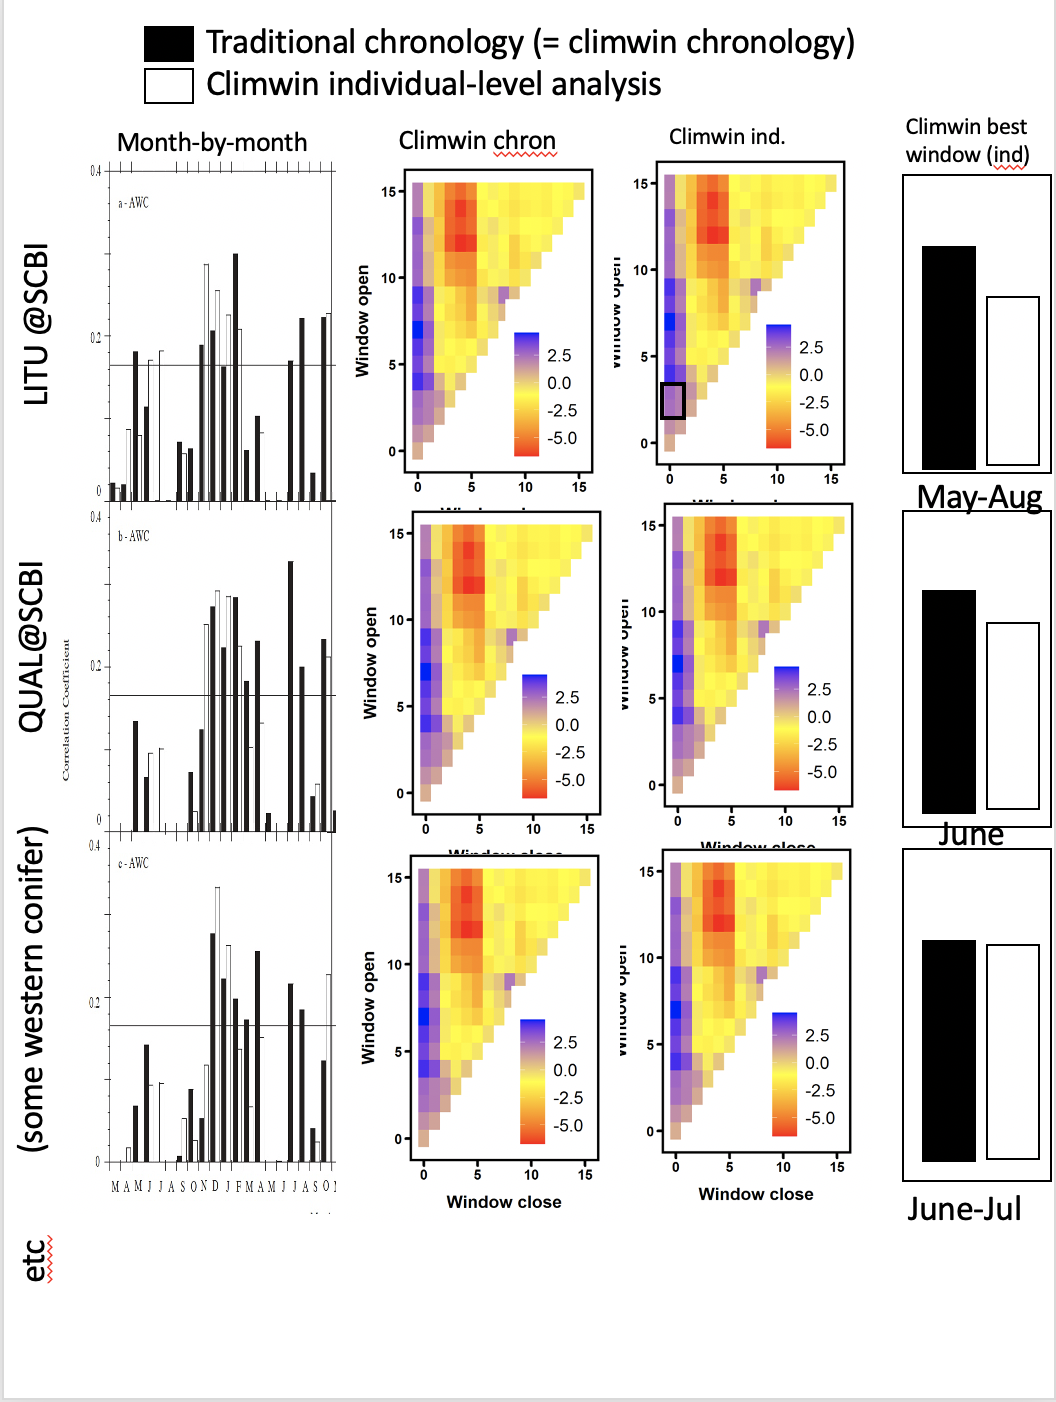
\includegraphics[width=0.7\textwidth,height=\textheight]{tables_figures/mock_comparison_traditional_method.png}
\caption{\textbf{Figure S1 \textbar{} (Comparison of traditional
approaches with ours).} (THIS FIGURE IS JUST A MOCK-UP --NOT REAL DATA.
REAL FIGURE WILL INCLUDE 3-4 COMMONLY STUDIED SPECIES FROM DIFFERENT
SITES.)}
\end{figure}

\newpage

\hypertarget{figure-s2.-comparison-of-climwin-output-across-growth-metrics-for-the-temperature-variable-group-at-little-tesuque-new-mexico-usa}{%
\subsection{Figure S2. Comparison of climwin output across growth
metrics for the temperature variable group at Little Tesuque (New
Mexico,
USA)}\label{figure-s2.-comparison-of-climwin-output-across-growth-metrics-for-the-temperature-variable-group-at-little-tesuque-new-mexico-usa}}

\begin{figure}
\centering
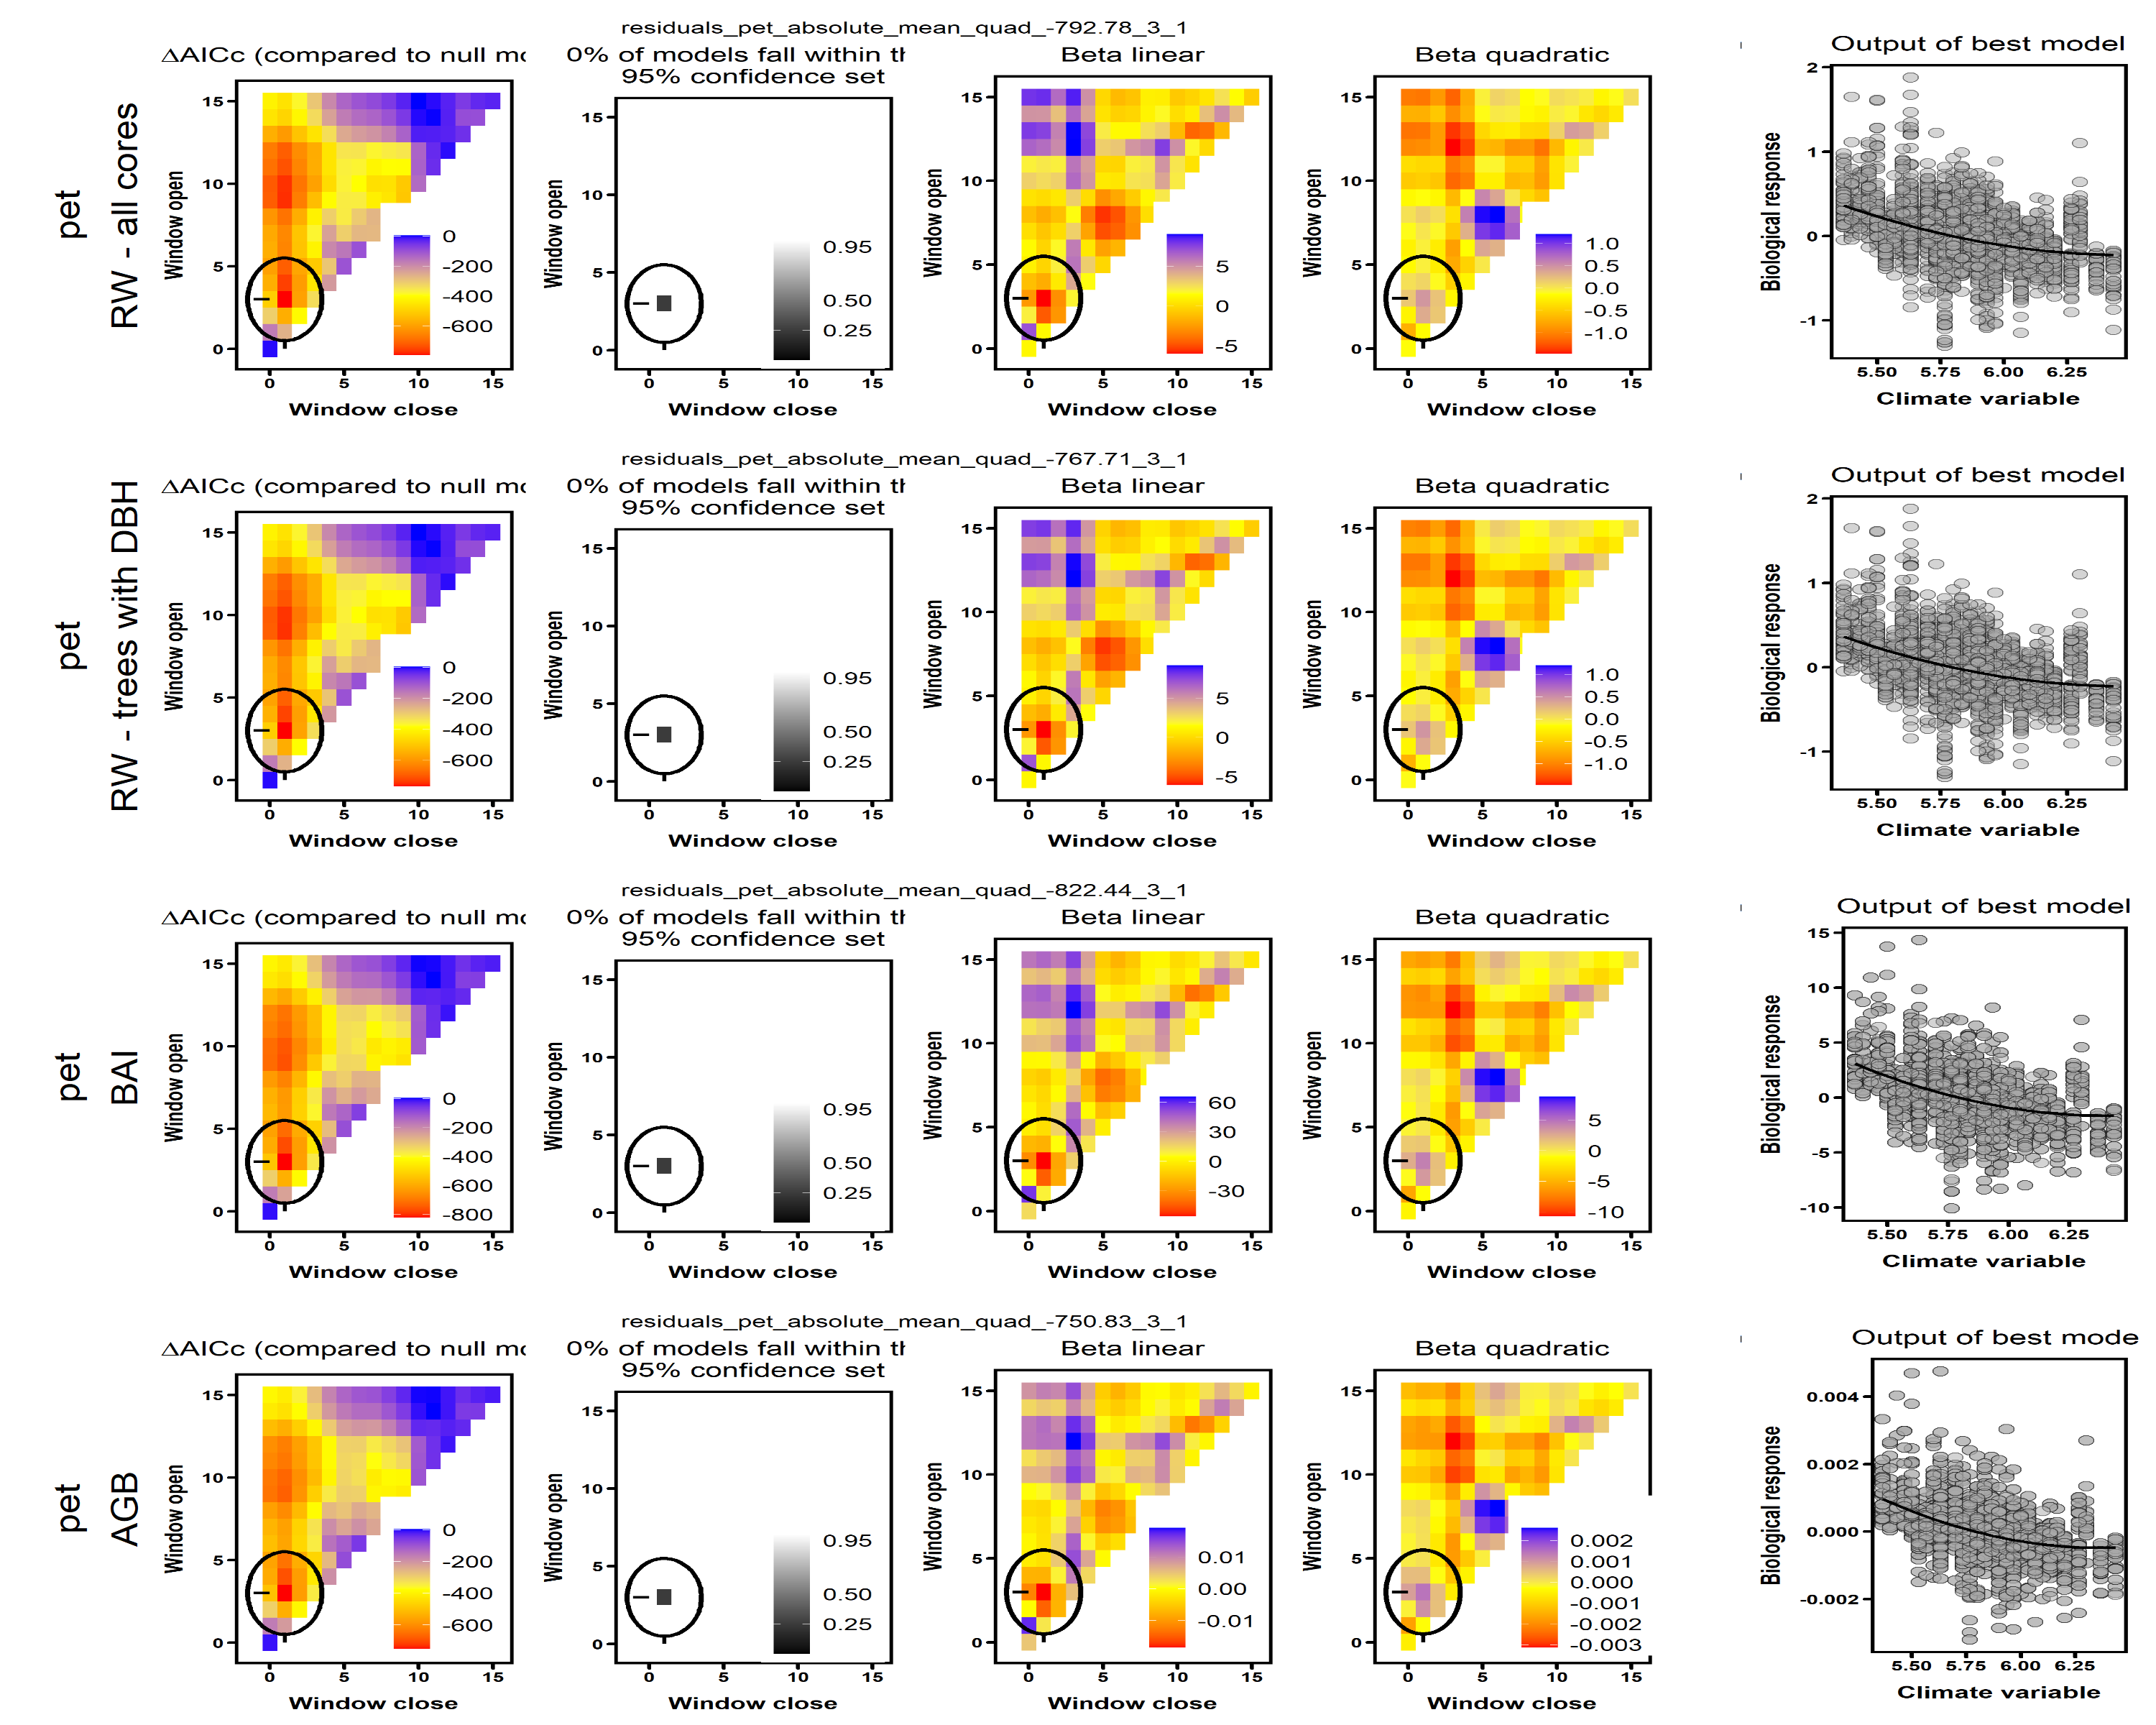
\includegraphics{/Users/kteixeira/Dropbox (Smithsonian)/GitHub/EcoClimLab/ForestGEO-climate-sensitivity/results/climwin_plots_combined/NewMexico_pet.png}
\caption{\textbf{Figure S2 \textbar{} Comparison of climwin output
across growth metrics for the temperature variable group at Little
Tesuque (New Mexico, USA).} Here, \emph{climwin} identified potential
evapotranspiration (\(PET\)) as the strongest climate variable across
all three metrics of growth (\(\Delta r\), BAI, \(\Delta AGB\)) and
regardless of whether all cores were included in the analysis, or only
those for which DBH could be reconstructed (\(\Delta r\)-trees with
\(DBH\), BAI, \(\Delta AGB\)).)}
\end{figure}

\newpage

\hypertarget{figure-s3.-comparison-of-climwin-output-across-growth-metrics-for-the-precipitation-variable-group-at-little-tesuque-new-mexico-usa}{%
\subsection{Figure S3. Comparison of climwin output across growth
metrics for the precipitation variable group at Little Tesuque (New
Mexico,
USA)}\label{figure-s3.-comparison-of-climwin-output-across-growth-metrics-for-the-precipitation-variable-group-at-little-tesuque-new-mexico-usa}}

\begin{figure}
\centering
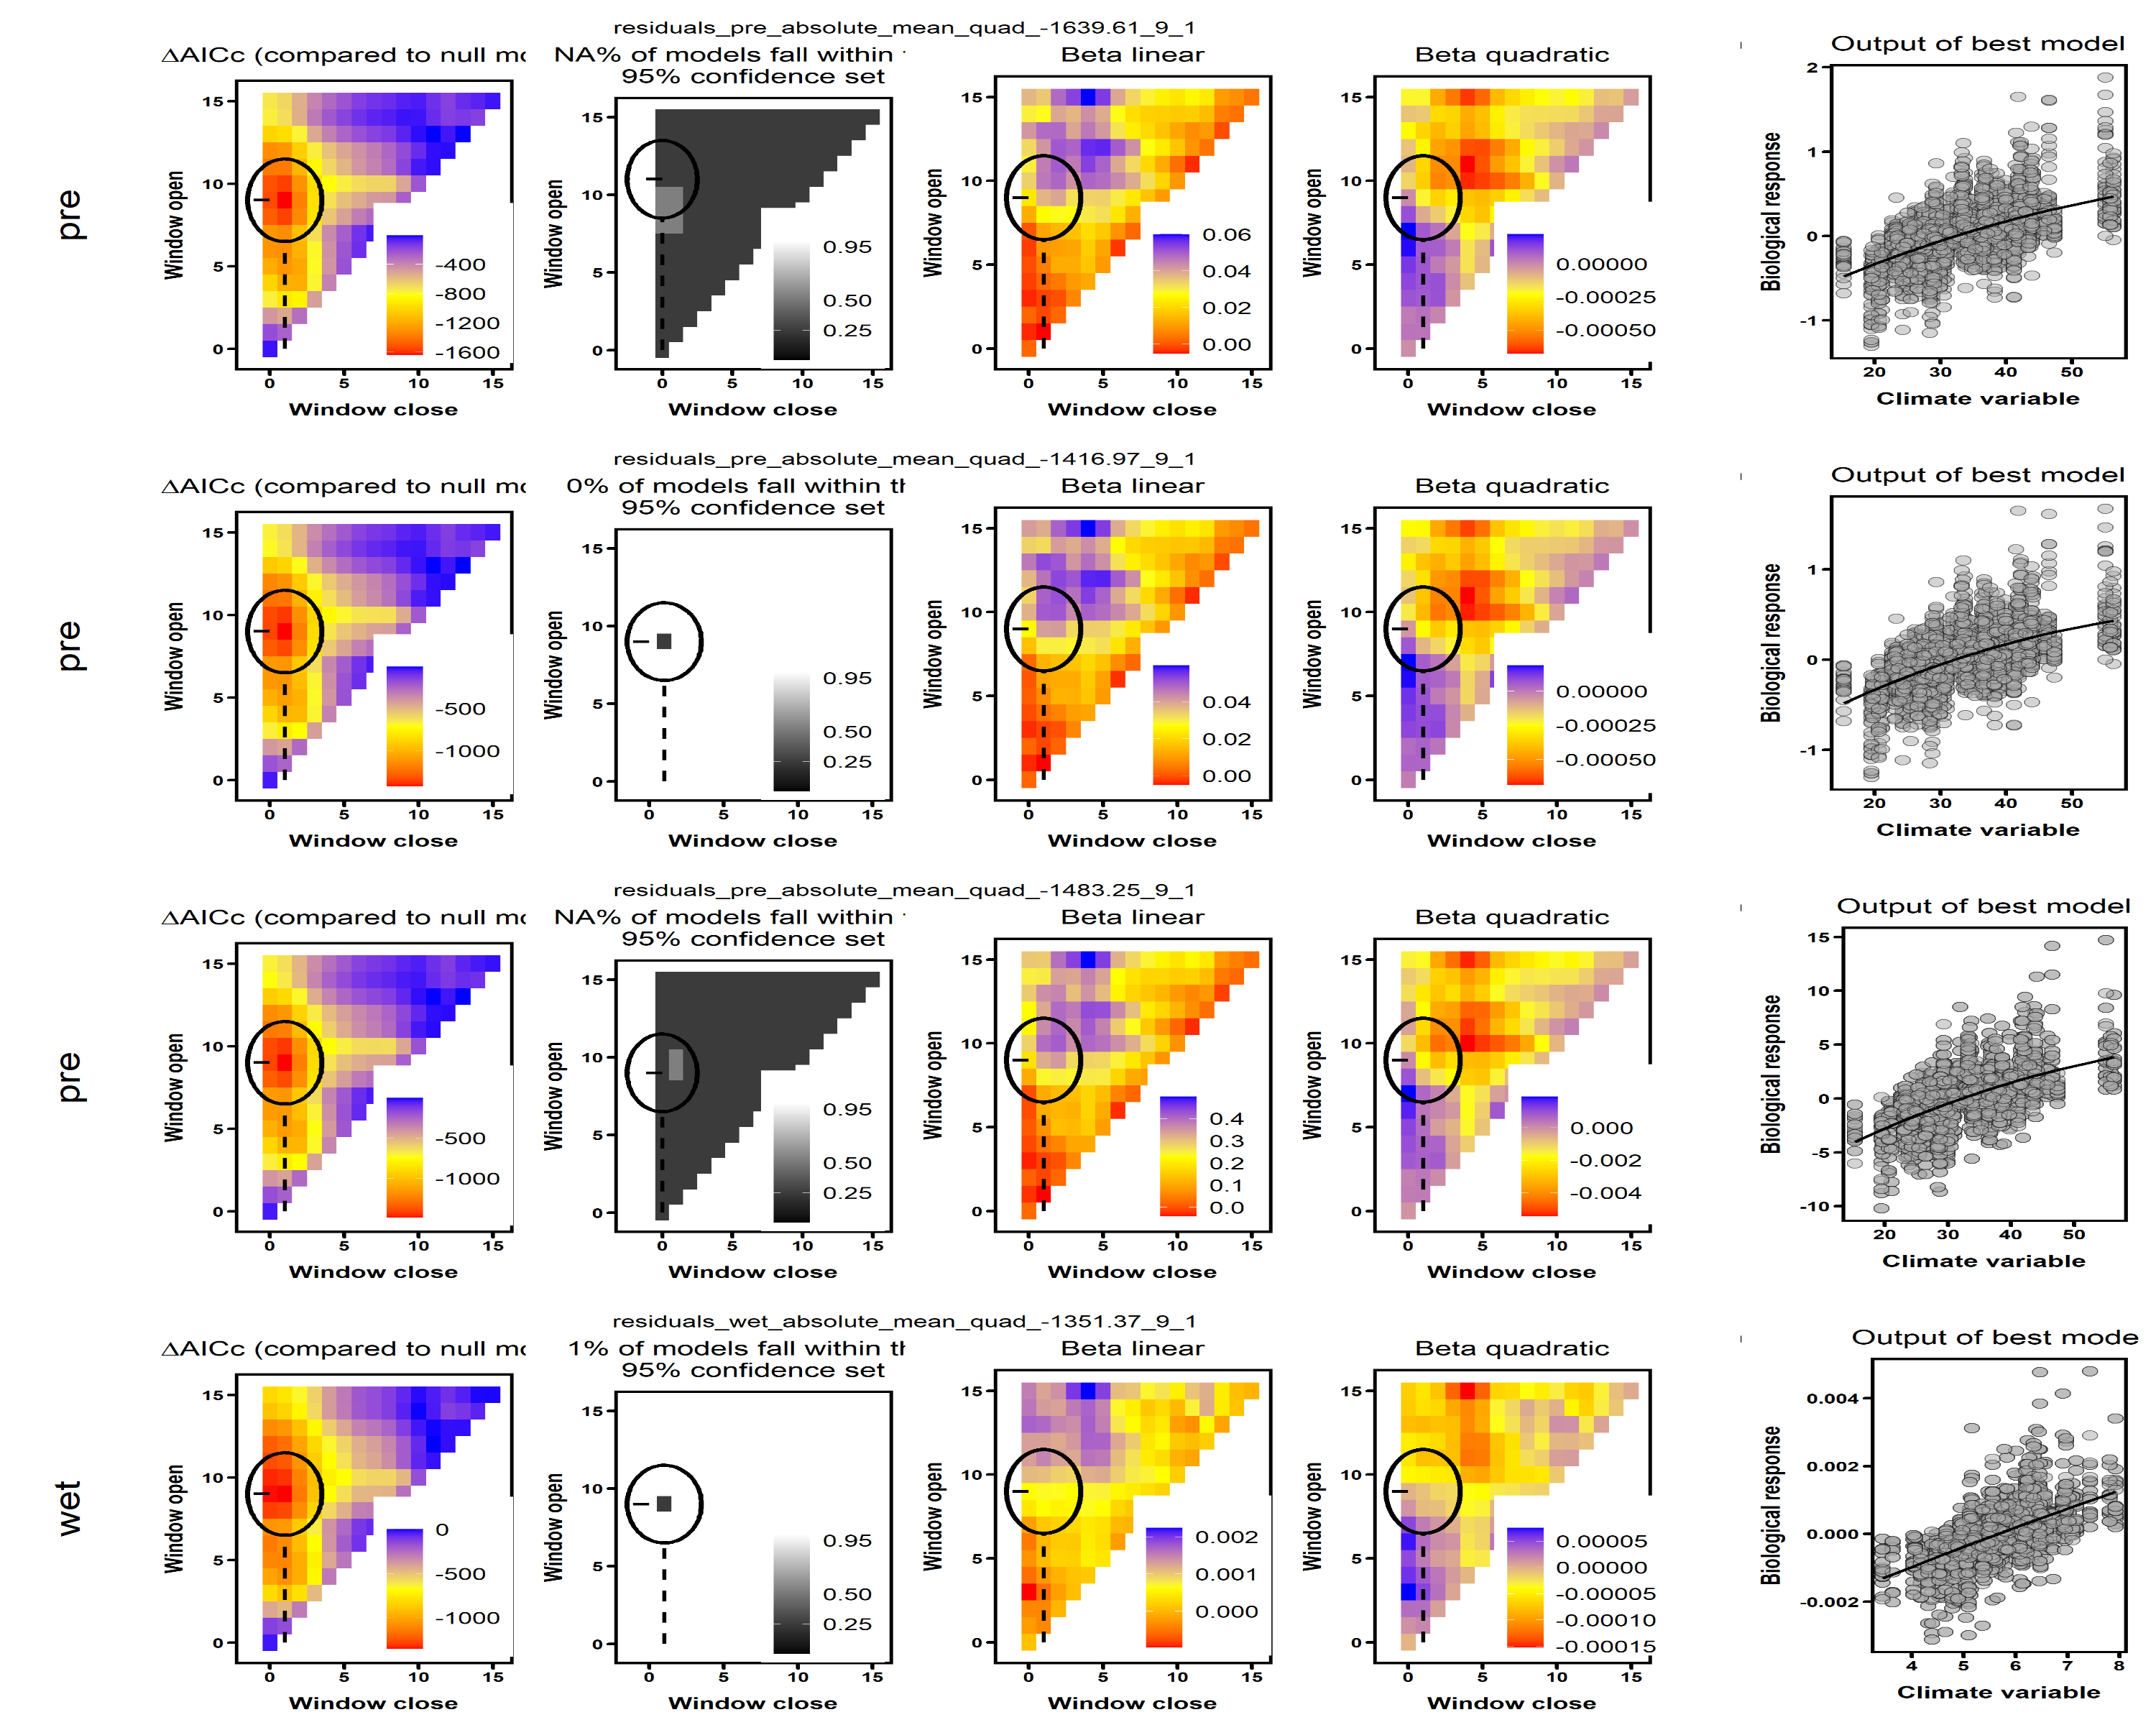
\includegraphics{/Users/kteixeira/Dropbox (Smithsonian)/GitHub/EcoClimLab/ForestGEO-climate-sensitivity/results/climwin_plots_combined/NewMexico_wet_pre.png}
\caption{\textbf{Figure S3 \textbar{} Comparison of climwin output
across growth metrics for the precipitation variable group at Little
Tesuque (New Mexico, USA).} Here, \emph{climwin} identified
precipitation (\(PPT\)) as the strongest climate variable for
\(\Delta r\) and \(BAI\), but precipitation day frequency (\(PDF\)) as
the strongest climate variable for \(\Delta AGB\).}
\end{figure}

\newpage

\hypertarget{figure-s4.-comparison-of-climwin-output-across-growth-metrics-for-the-precipitation-variable-group-at-harvard-forest-massachusetts-usa}{%
\subsection{Figure S4. Comparison of climwin output across growth
metrics for the precipitation variable group at Harvard Forest
(Massachusetts,
USA)}\label{figure-s4.-comparison-of-climwin-output-across-growth-metrics-for-the-precipitation-variable-group-at-harvard-forest-massachusetts-usa}}

\begin{figure}
\centering
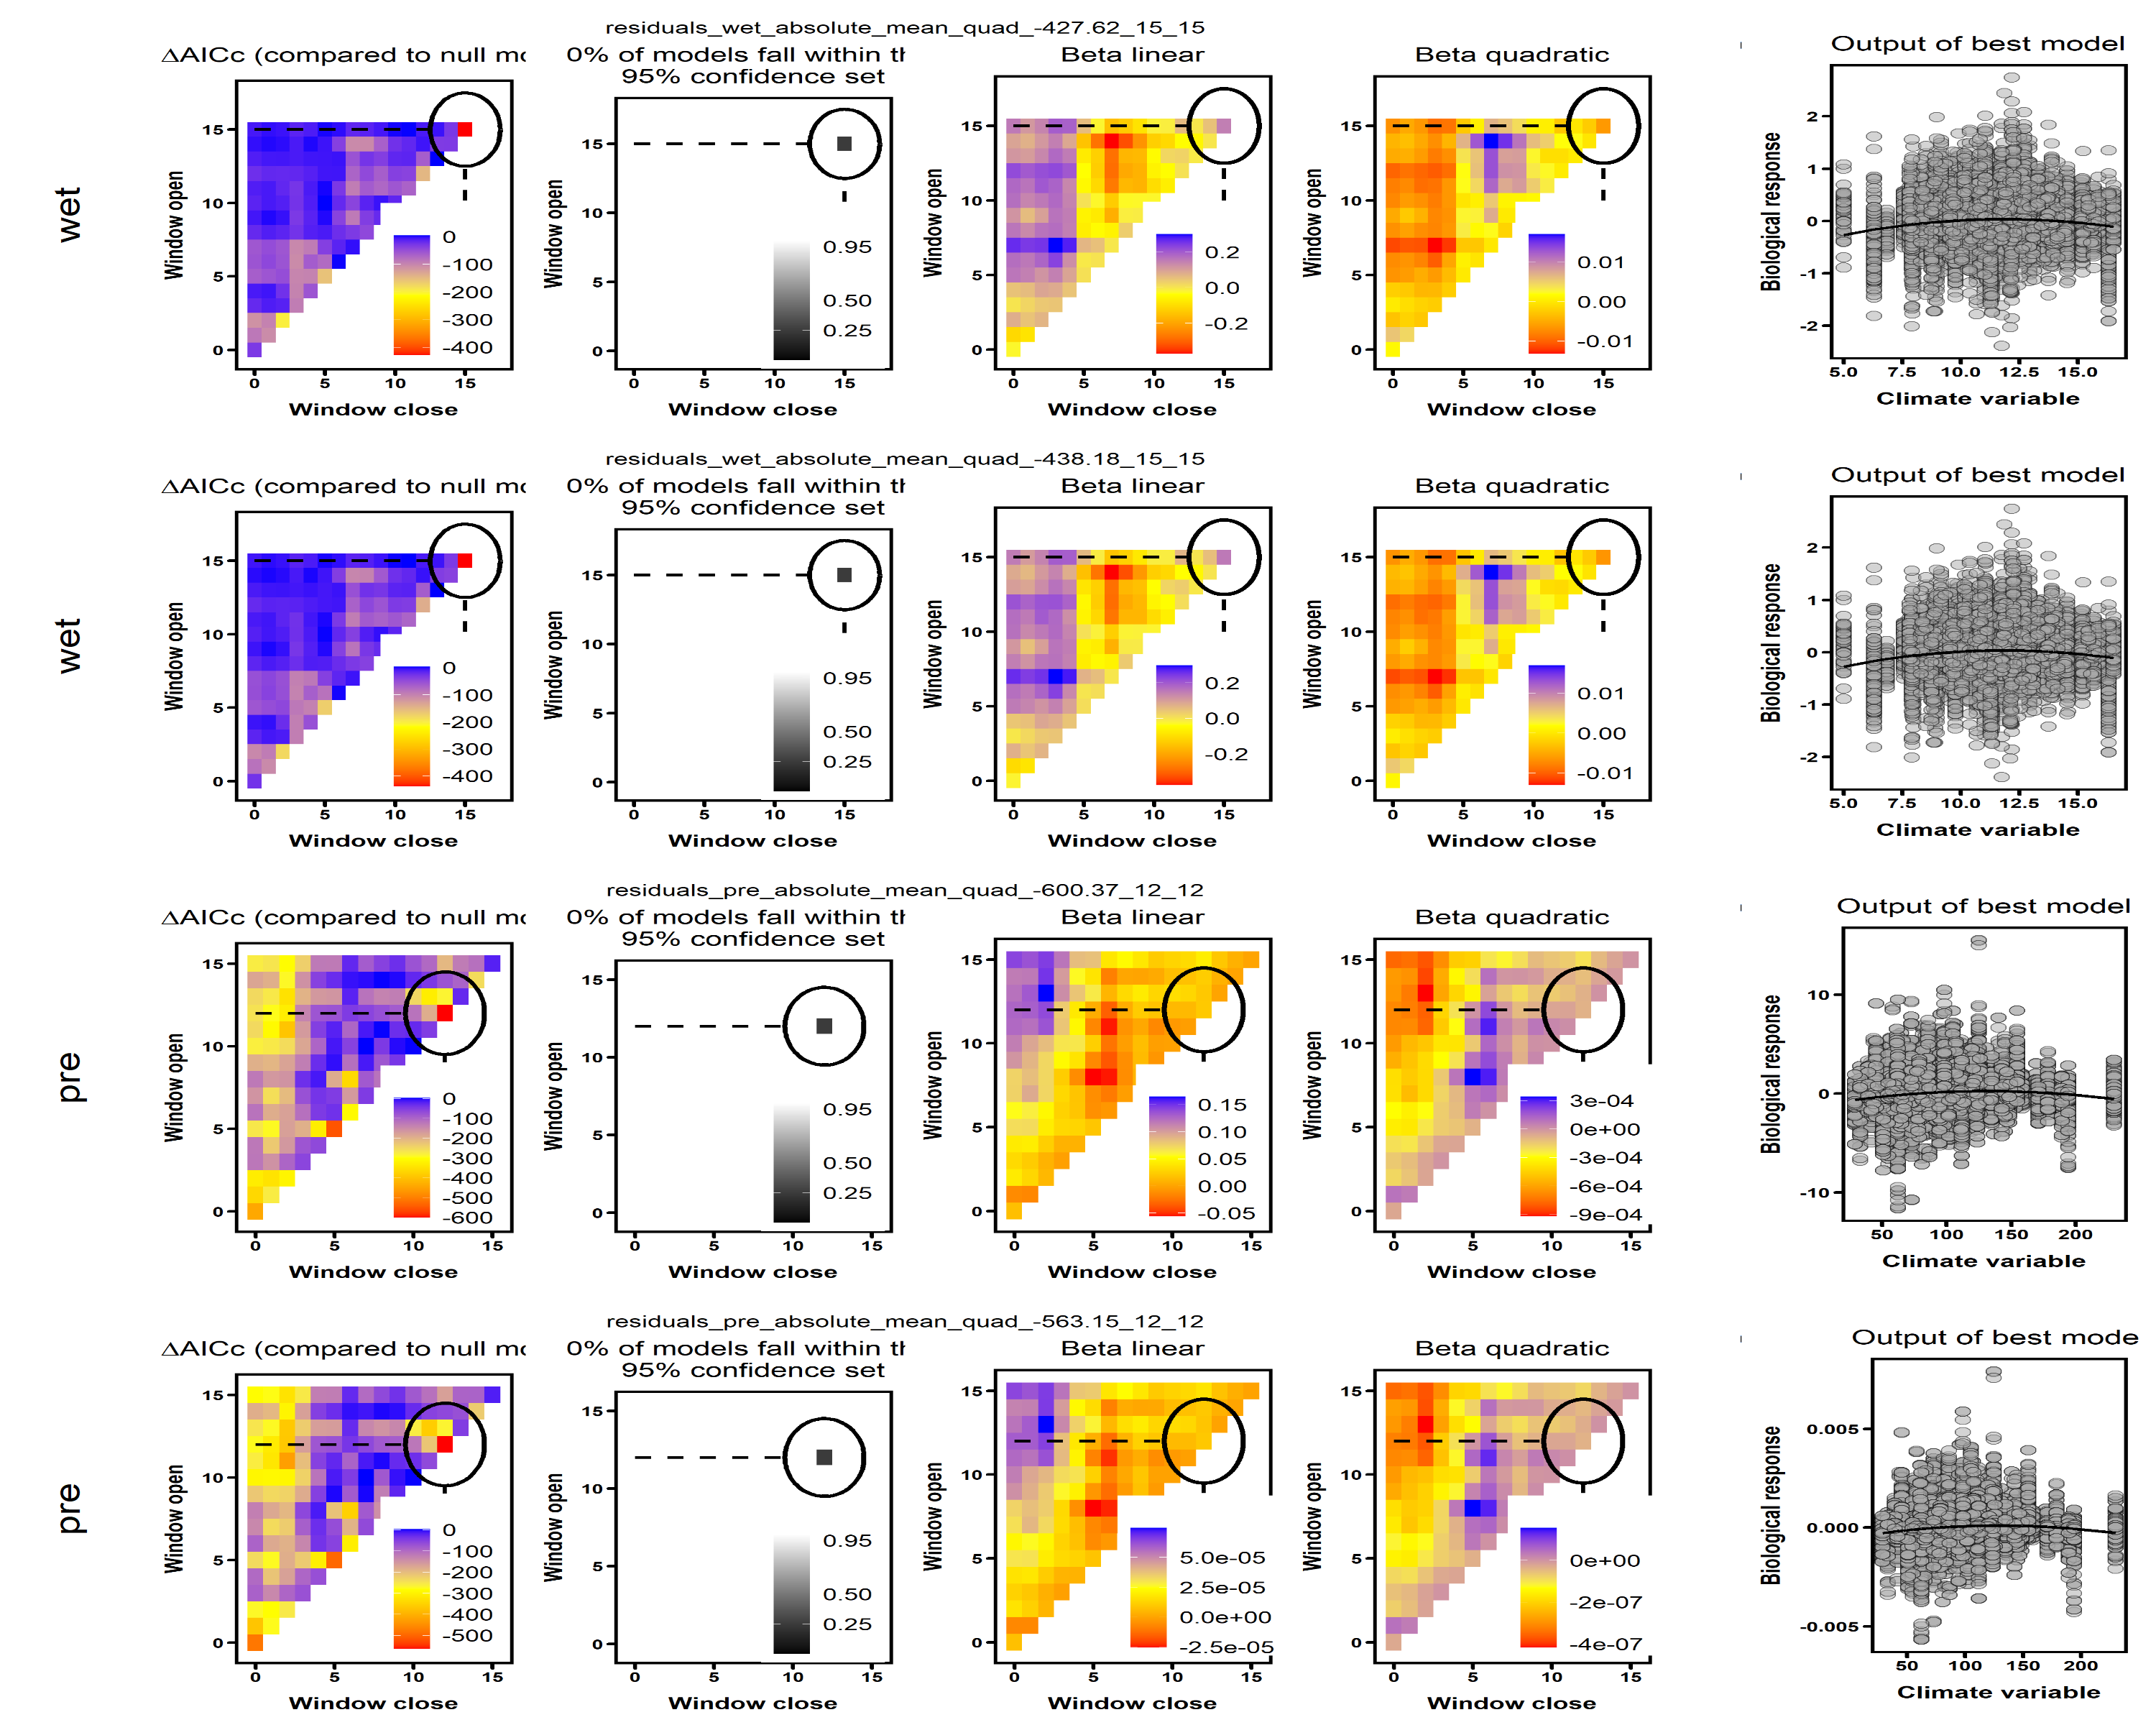
\includegraphics{/Users/kteixeira/Dropbox (Smithsonian)/GitHub/EcoClimLab/ForestGEO-climate-sensitivity/results/climwin_plots_combined/HarvardForest_pre_wet.png}
\caption{\textbf{Figure S4 \textbar{} Comparison of climwin output
across growth metrics for the precipitation variable group at Harvard
Forest (Massachusetts, USA).} Here, \emph{climwin} identified
precipitation frequency (\(PDF\)) as the strongest climate variable for
\(\Delta r\), but precipitation amount (\(PPT\)) as the strongest
climate variable for \(BAI\) and \(\Delta AGB\). The optimal time window
(circled) also differed across growth metrics.}
\end{figure}

\newpage

\hypertarget{figure-s5.-best-gls-models-for-barro-colorado-island-panama}{%
\subsection{Figure S5. Best GLS models for Barro Colorado Island
(Panama)}\label{figure-s5.-best-gls-models-for-barro-colorado-island-panama}}

\begin{figure}
\centering
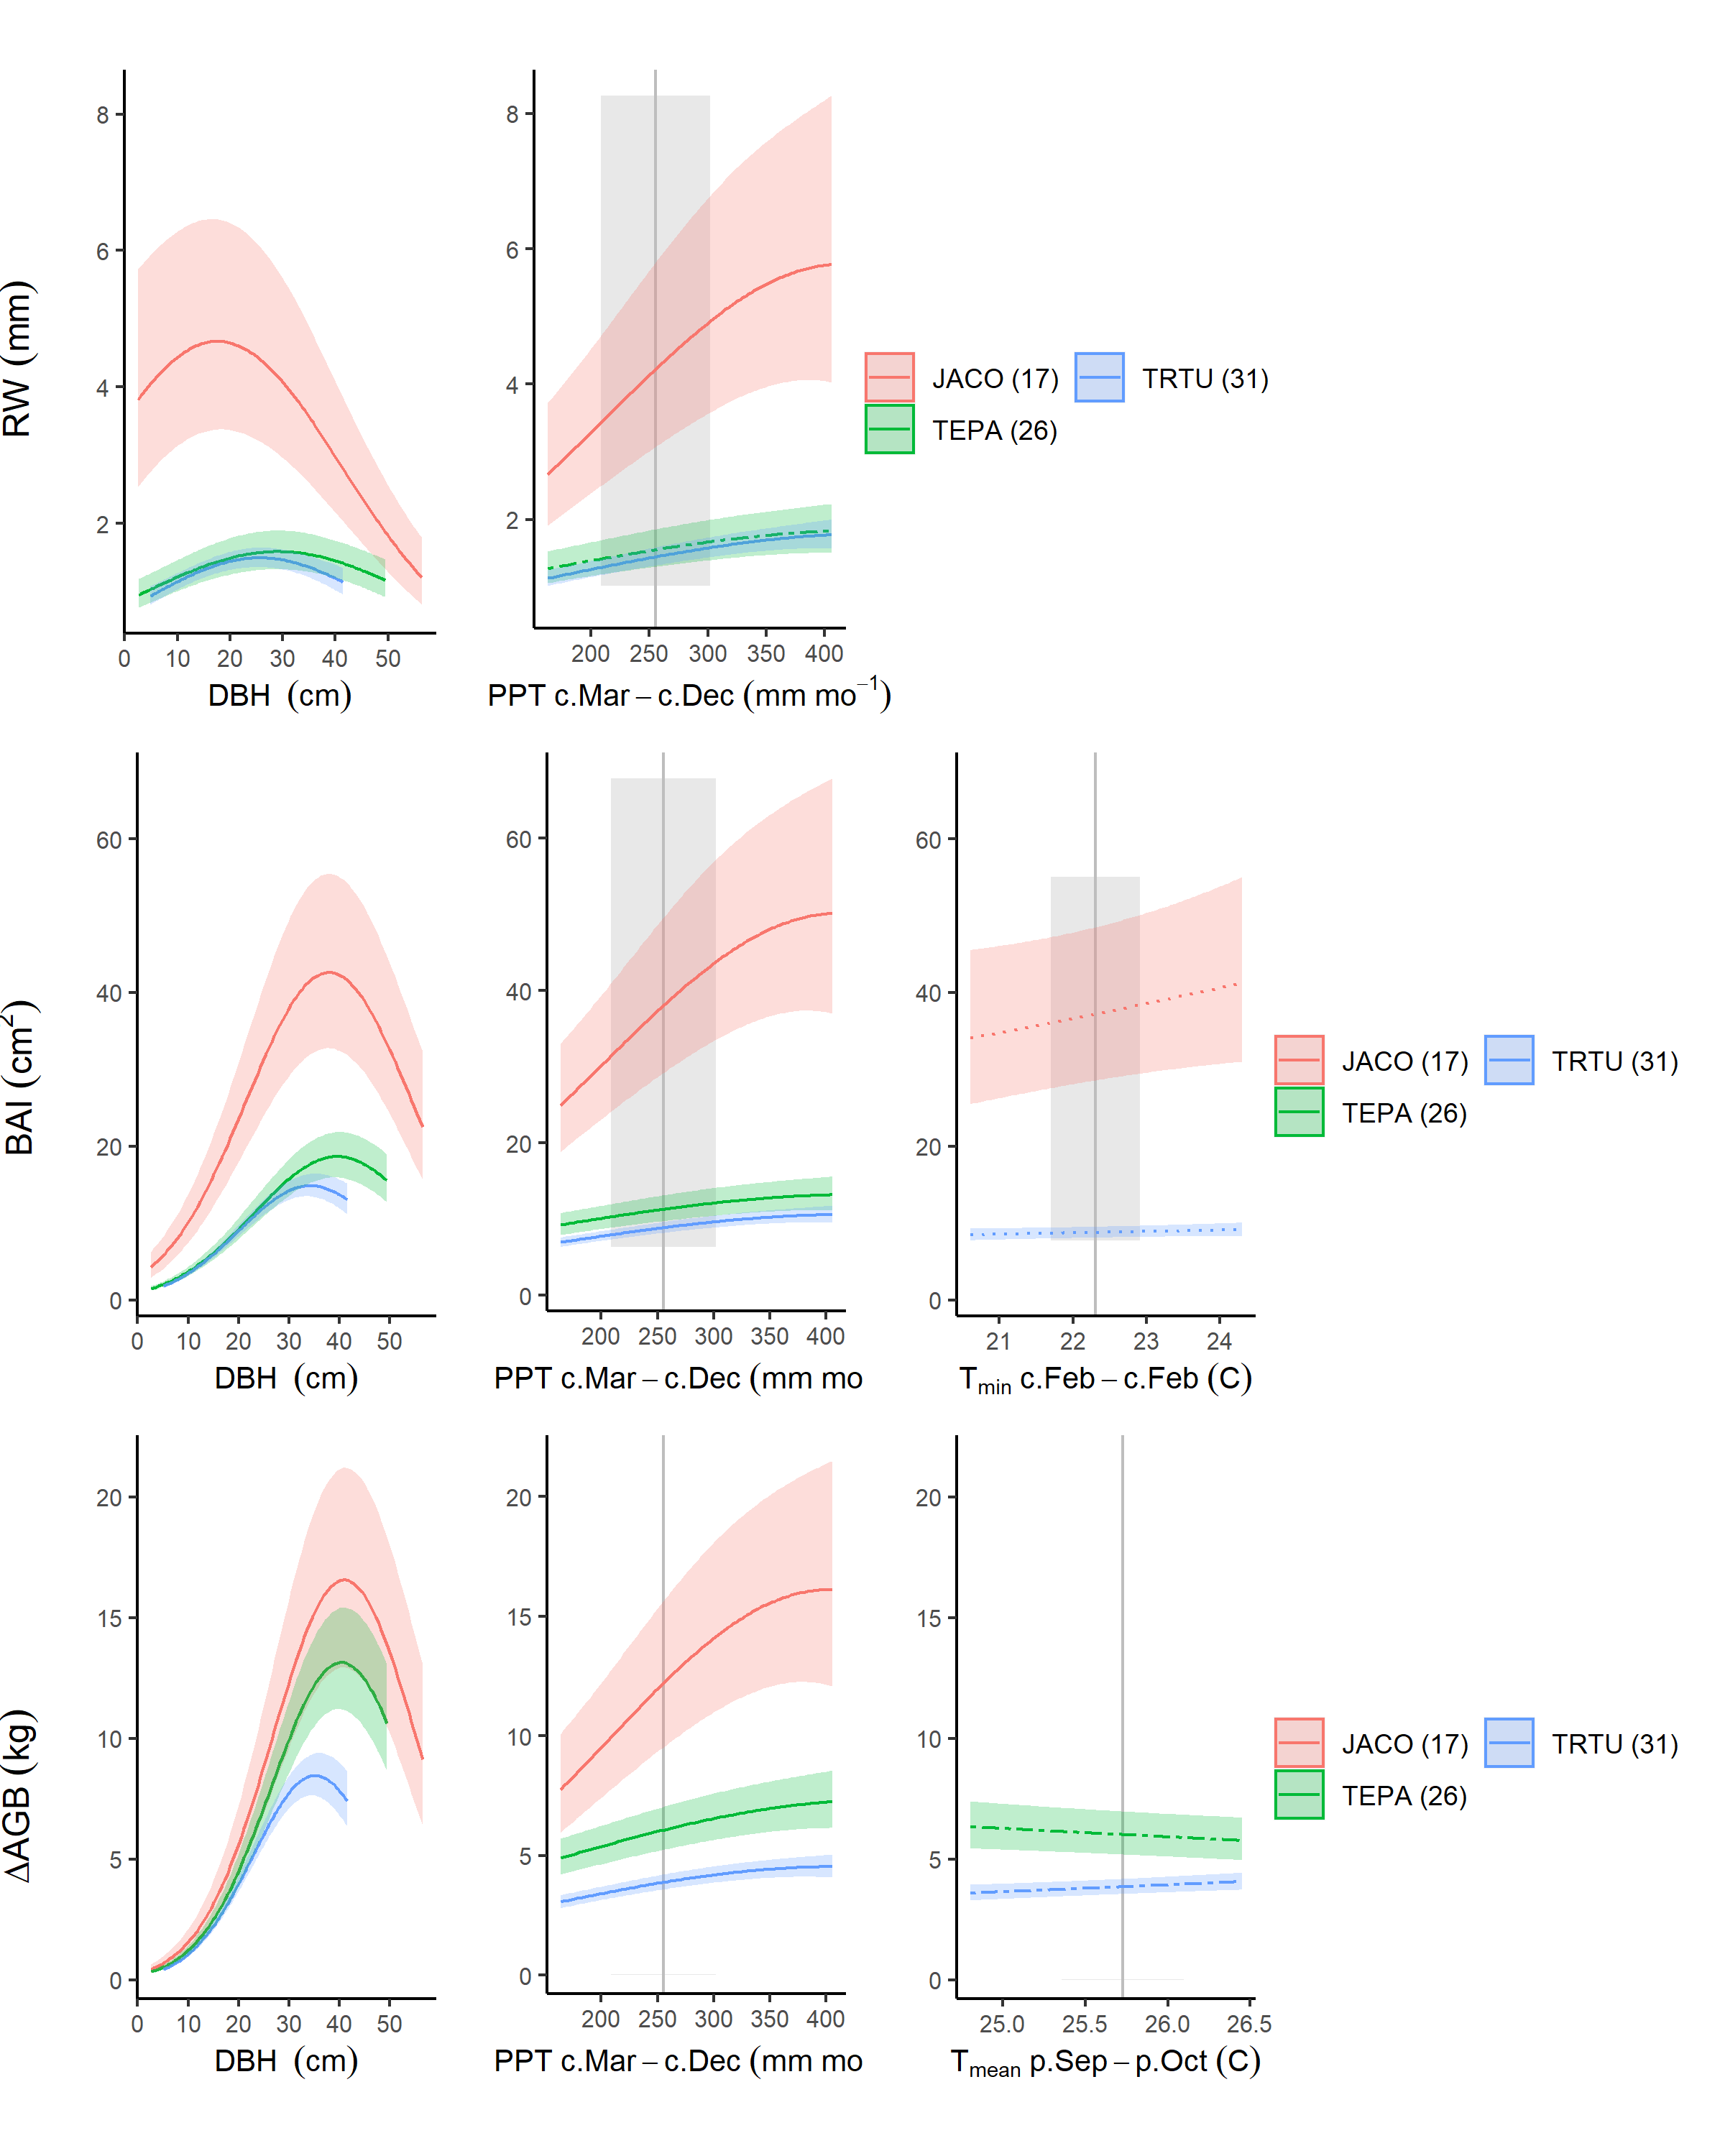
\includegraphics[width=0.75\textwidth,height=\textheight]{/Users/kteixeira/Dropbox (Smithsonian)/GitHub/EcoClimLab/ForestGEO-climate-sensitivity/results/composite_plots/BCI.png}
\caption{\textbf{Figure S5 \textbar{} Best GLS models for Barro Colorado
Island (Panama) for all three growth metrics: \(\Delta r\), \(BAI\), and
\(\Delta AGB\).} Precipitation and temperature group variables are as
selected by \emph{climwin} (p=previous year, c=current year). For each
species, relationships are plotted if included in top model, with
best-fit polynomials plotted with solid lines when both first- and
second-order terms are signficant, dashed lines when only one term is
signficant, and dotted lines when neither is signficant. Transparent
ribbons indicate 95\% confidence intervals. Vertical grey lines indicate
the long-term mean for the climate variable, shading indicates 1 SD.}
\end{figure}

\newpage

\hypertarget{figure-s6.-best-gls-models-for-huai-kha-khaeng-thailand}{%
\subsection{Figure S6. Best GLS models for Huai Kha Khaeng
(Thailand)}\label{figure-s6.-best-gls-models-for-huai-kha-khaeng-thailand}}

\begin{figure}
\centering
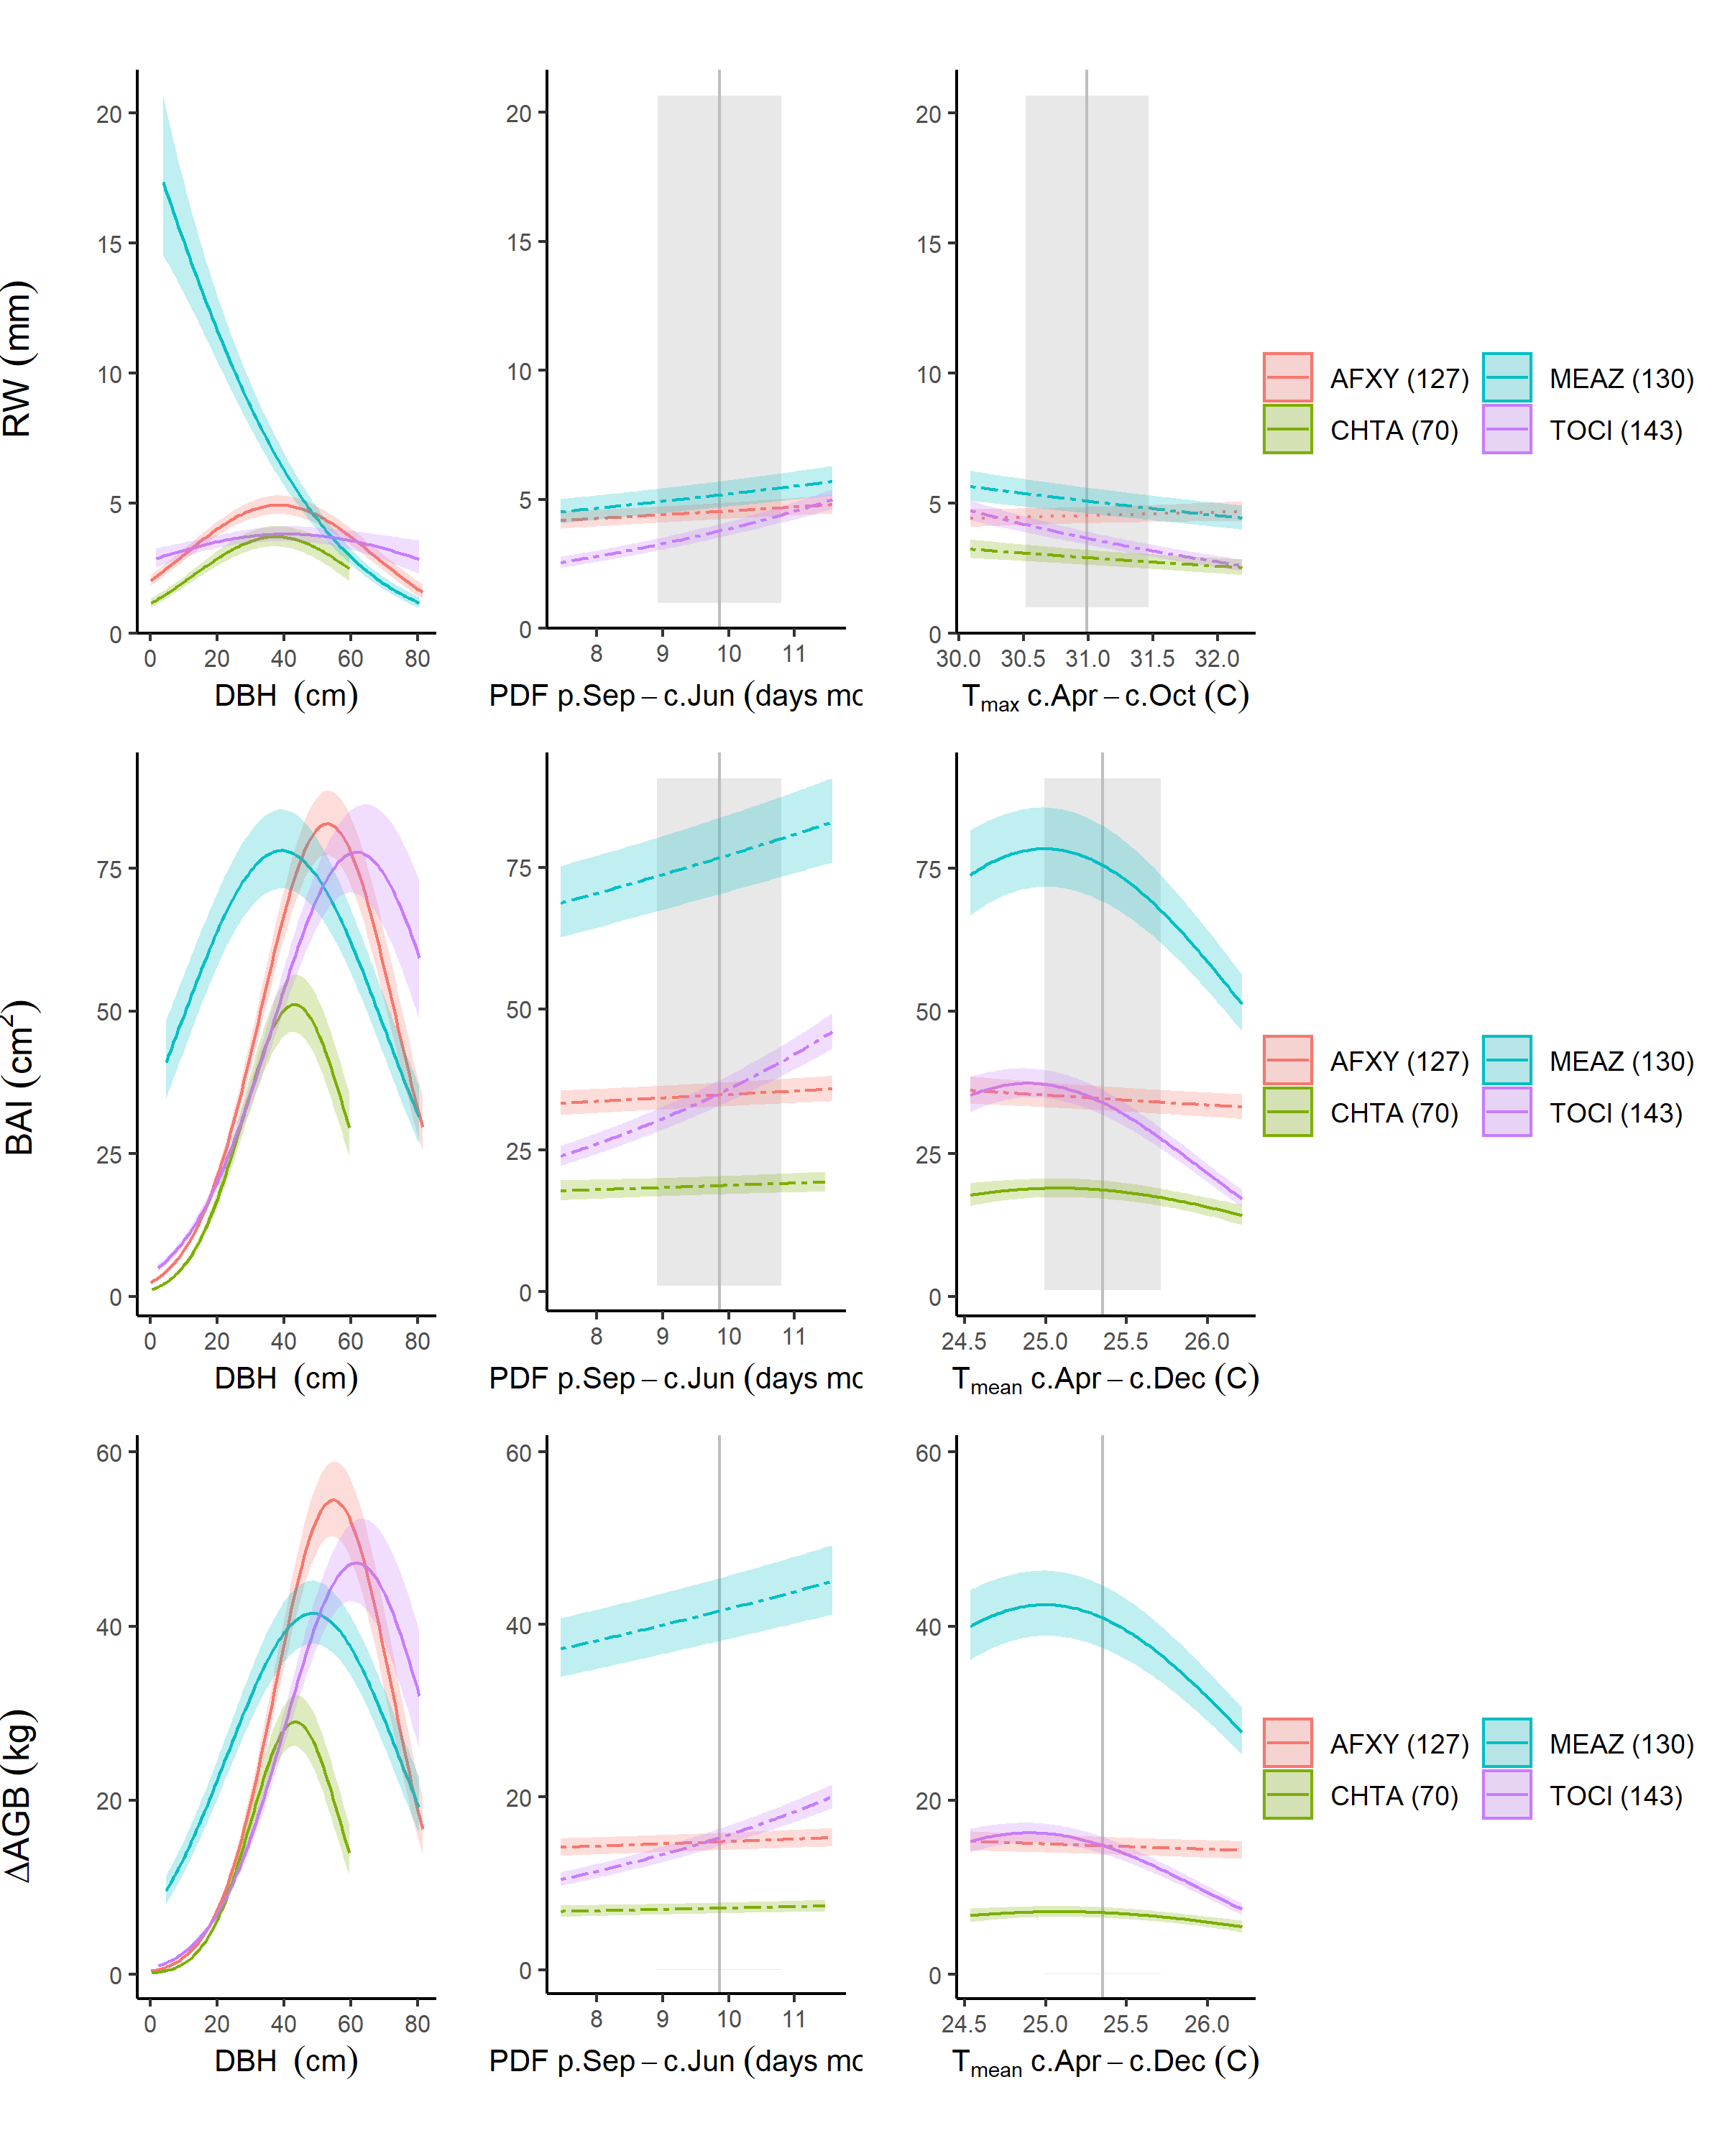
\includegraphics[width=0.75\textwidth,height=\textheight]{/Users/kteixeira/Dropbox (Smithsonian)/GitHub/EcoClimLab/ForestGEO-climate-sensitivity/results/composite_plots/HKK.png}
\caption{\textbf{Figure S6 \textbar{} Best GLS models for Huai Kha
Khaeng (Thailand) for all three growth metrics: \(\Delta r\), \(BAI\),
and \(\Delta AGB\).} Precipitation and temperature group variables are
as selected by \emph{climwin} (p=previous year, c=current year). For
each species, relationships are plotted if included in top model, with
best-fit polynomials plotted with solid lines when both first- and
second-order terms are signficant, dashed lines when only one term is
signficant, and dotted lines when neither is signficant. Transparent
ribbons indicate 95\% confidence intervals. Vertical grey lines indicate
the long-term mean for the climate variable, shading indicates 1 SD.}
\end{figure}

\newpage

\hypertarget{figure-s7.-best-gls-models-for-little-tesuque-new-mexico-usa}{%
\subsection{Figure S7. Best GLS models for Little Tesuque (New Mexico,
USA)}\label{figure-s7.-best-gls-models-for-little-tesuque-new-mexico-usa}}

\begin{figure}
\centering
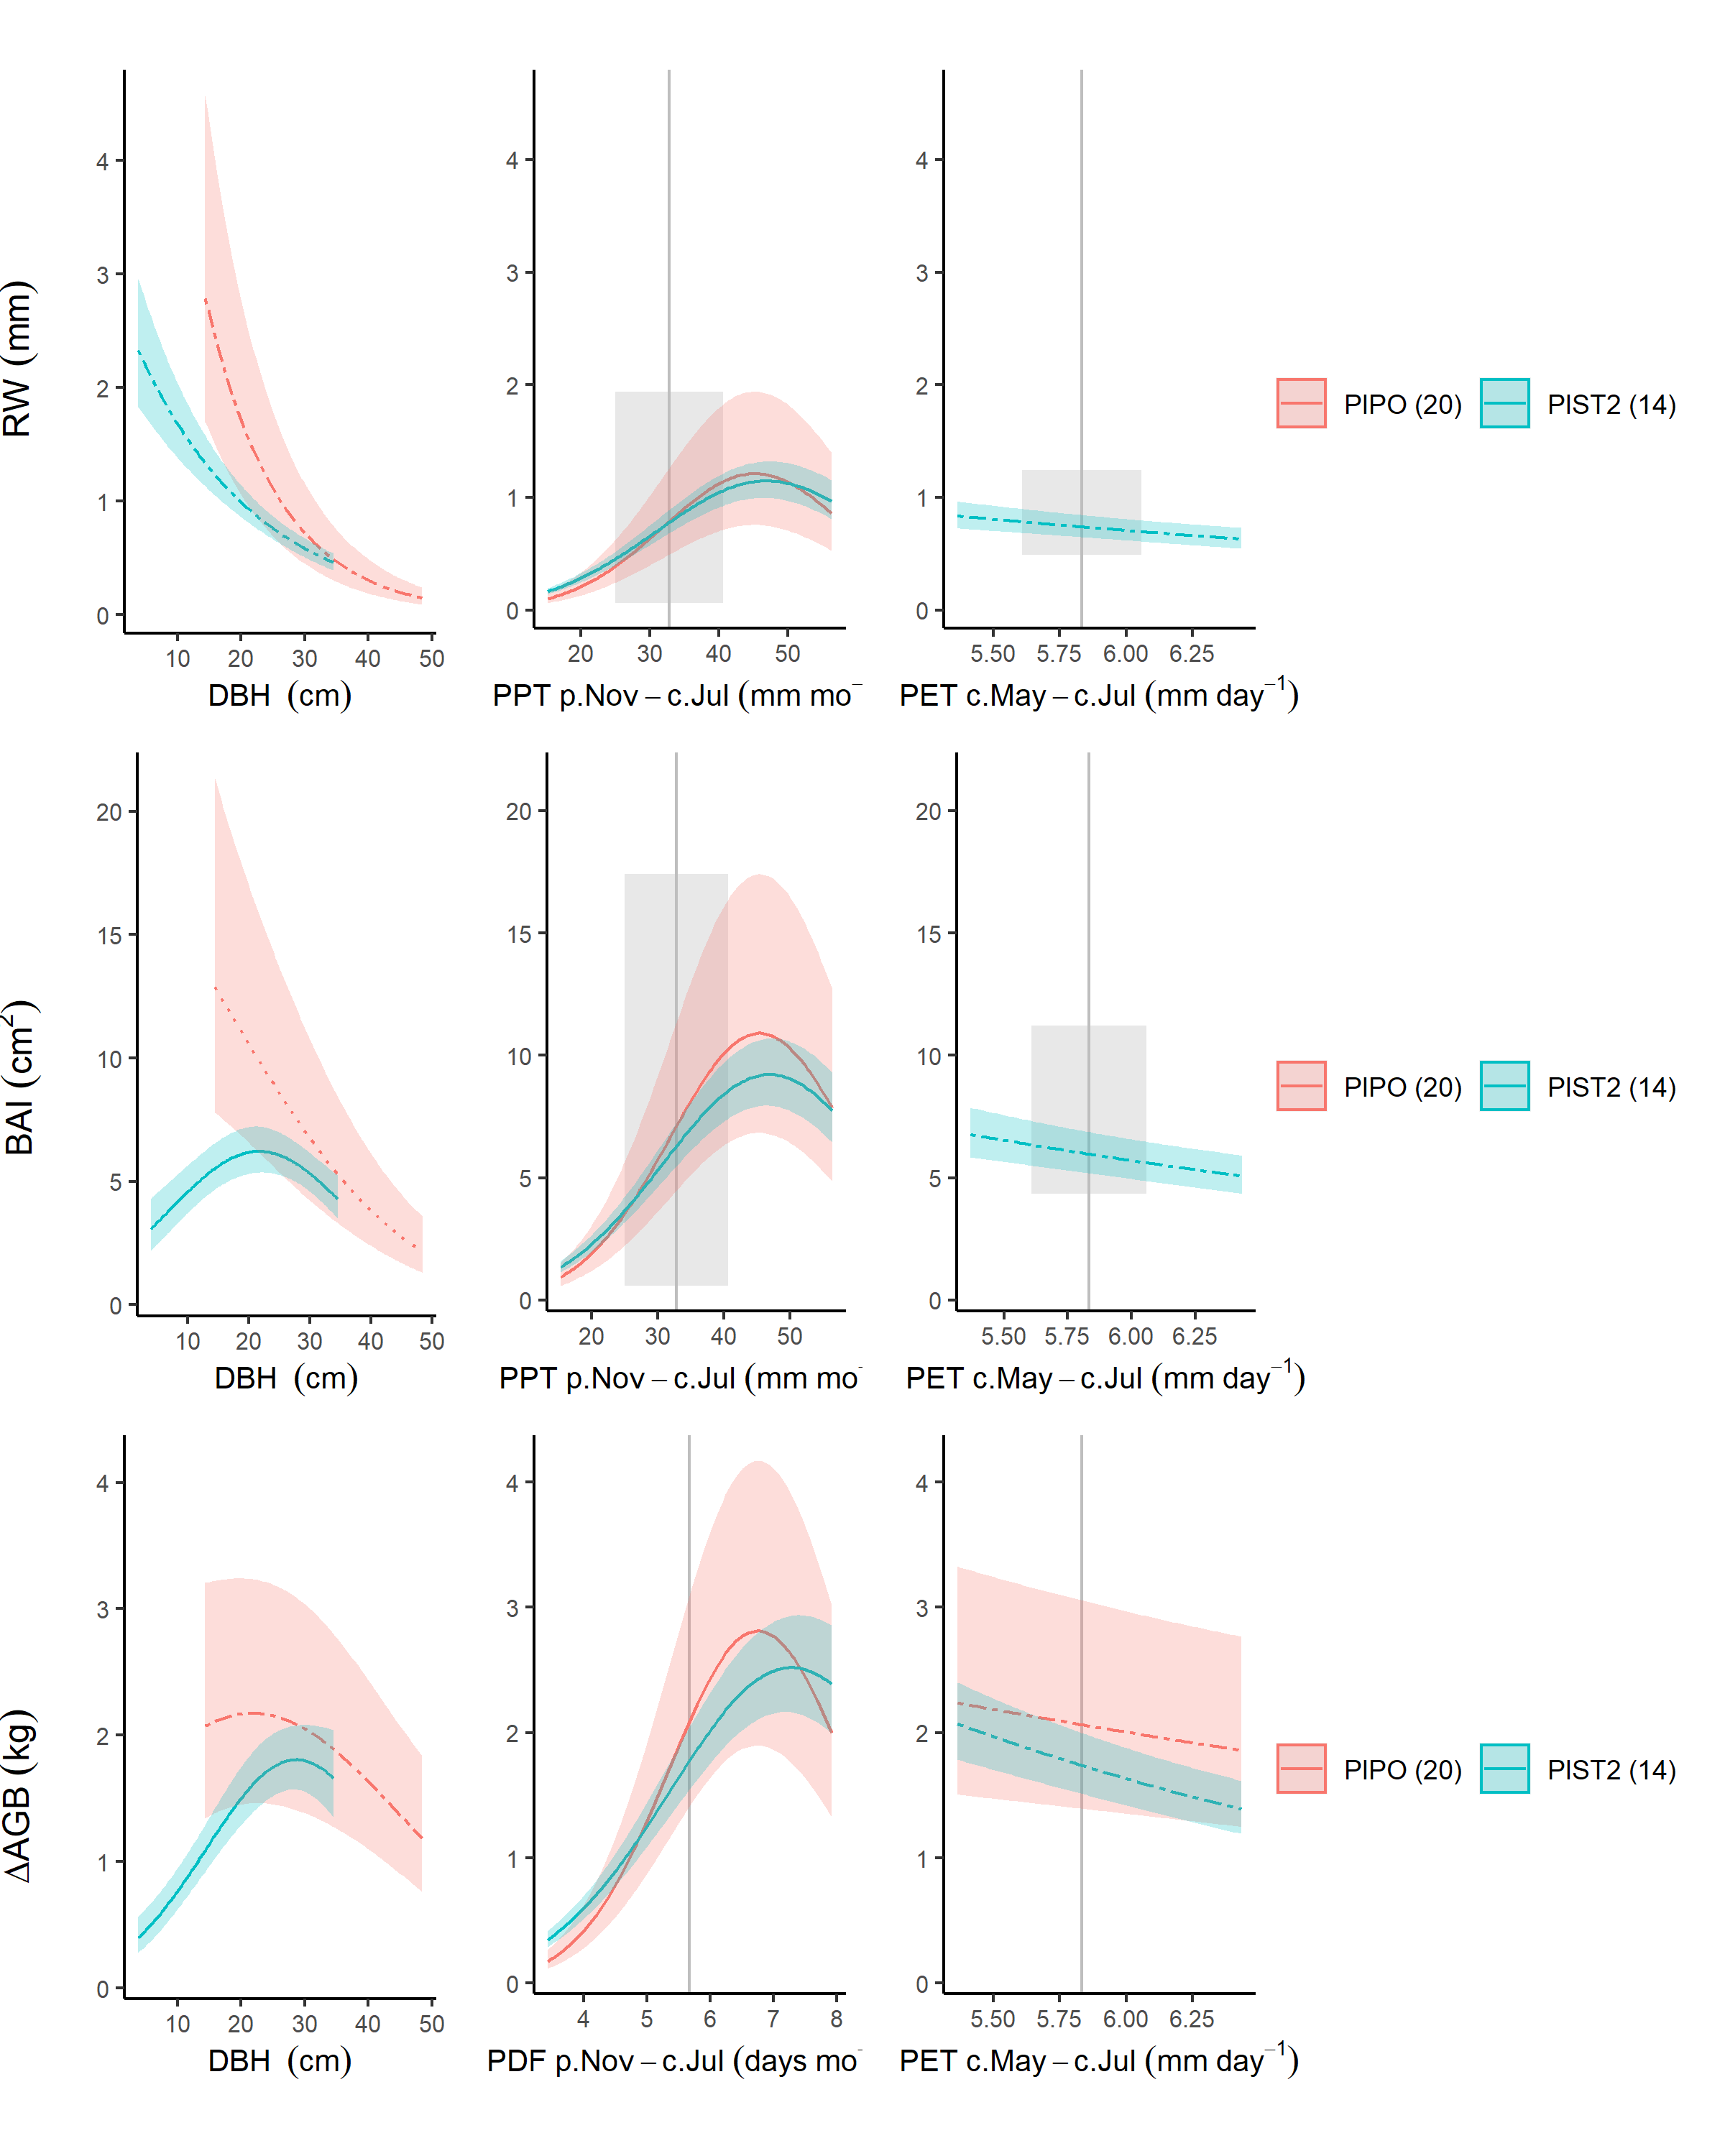
\includegraphics[width=0.75\textwidth,height=\textheight]{/Users/kteixeira/Dropbox (Smithsonian)/GitHub/EcoClimLab/ForestGEO-climate-sensitivity/results/composite_plots/NewMexico.png}
\caption{\textbf{Figure S7 \textbar{} Best GLS models for Little Tesuque
(New Mexico, USA) for all three growth metrics: \(\Delta r\), \(BAI\),
and \(\Delta AGB\).} Precipitation and temperature group variables are
as selected by \emph{climwin} (p=previous year, c=current year). For
each species, relationships are plotted if included in top model, with
best-fit polynomials plotted with solid lines when both first- and
second-order terms are signficant, dashed lines when only one term is
signficant, and dotted lines when neither is signficant. Transparent
ribbons indicate 95\% confidence intervals. Vertical grey lines indicate
the long-term mean for the climate variable, shading indicates 1 SD.}
\end{figure}

\newpage

\hypertarget{figure-s8.-best-gls-models-for-cedar-breaks-utah-usa}{%
\subsection{Figure S8. Best GLS models for Cedar Breaks (Utah,
USA)}\label{figure-s8.-best-gls-models-for-cedar-breaks-utah-usa}}

{[}\textbf{Figure S8 \textbar{} Best GLS models for Cedar Breaks (Utah,
USA) for all three growth metrics: \(\Delta r\), \(BAI\), and
\(\Delta AGB\).} Precipitation and temperature group variables are as
selected by \emph{climwin} (p=previous year, c=current year). For each
species, relationships are plotted if included in top model, with
best-fit polynomials plotted with solid lines when both first- and
second-order terms are signficant, dashed lines when only one term is
signficant, and dotted lines when neither is signficant. Transparent
ribbons indicate 95\% confidence intervals. Vertical grey lines indicate
the long-term mean for the climate variable, shading indicates 1 SD.{]}

\newpage

\hypertarget{figure-s9.-best-gls-models-for-scbi-virginia-usa}{%
\subsection{Figure S9. Best GLS models for SCBI (Virginia,
USA)}\label{figure-s9.-best-gls-models-for-scbi-virginia-usa}}

\begin{figure}
\centering
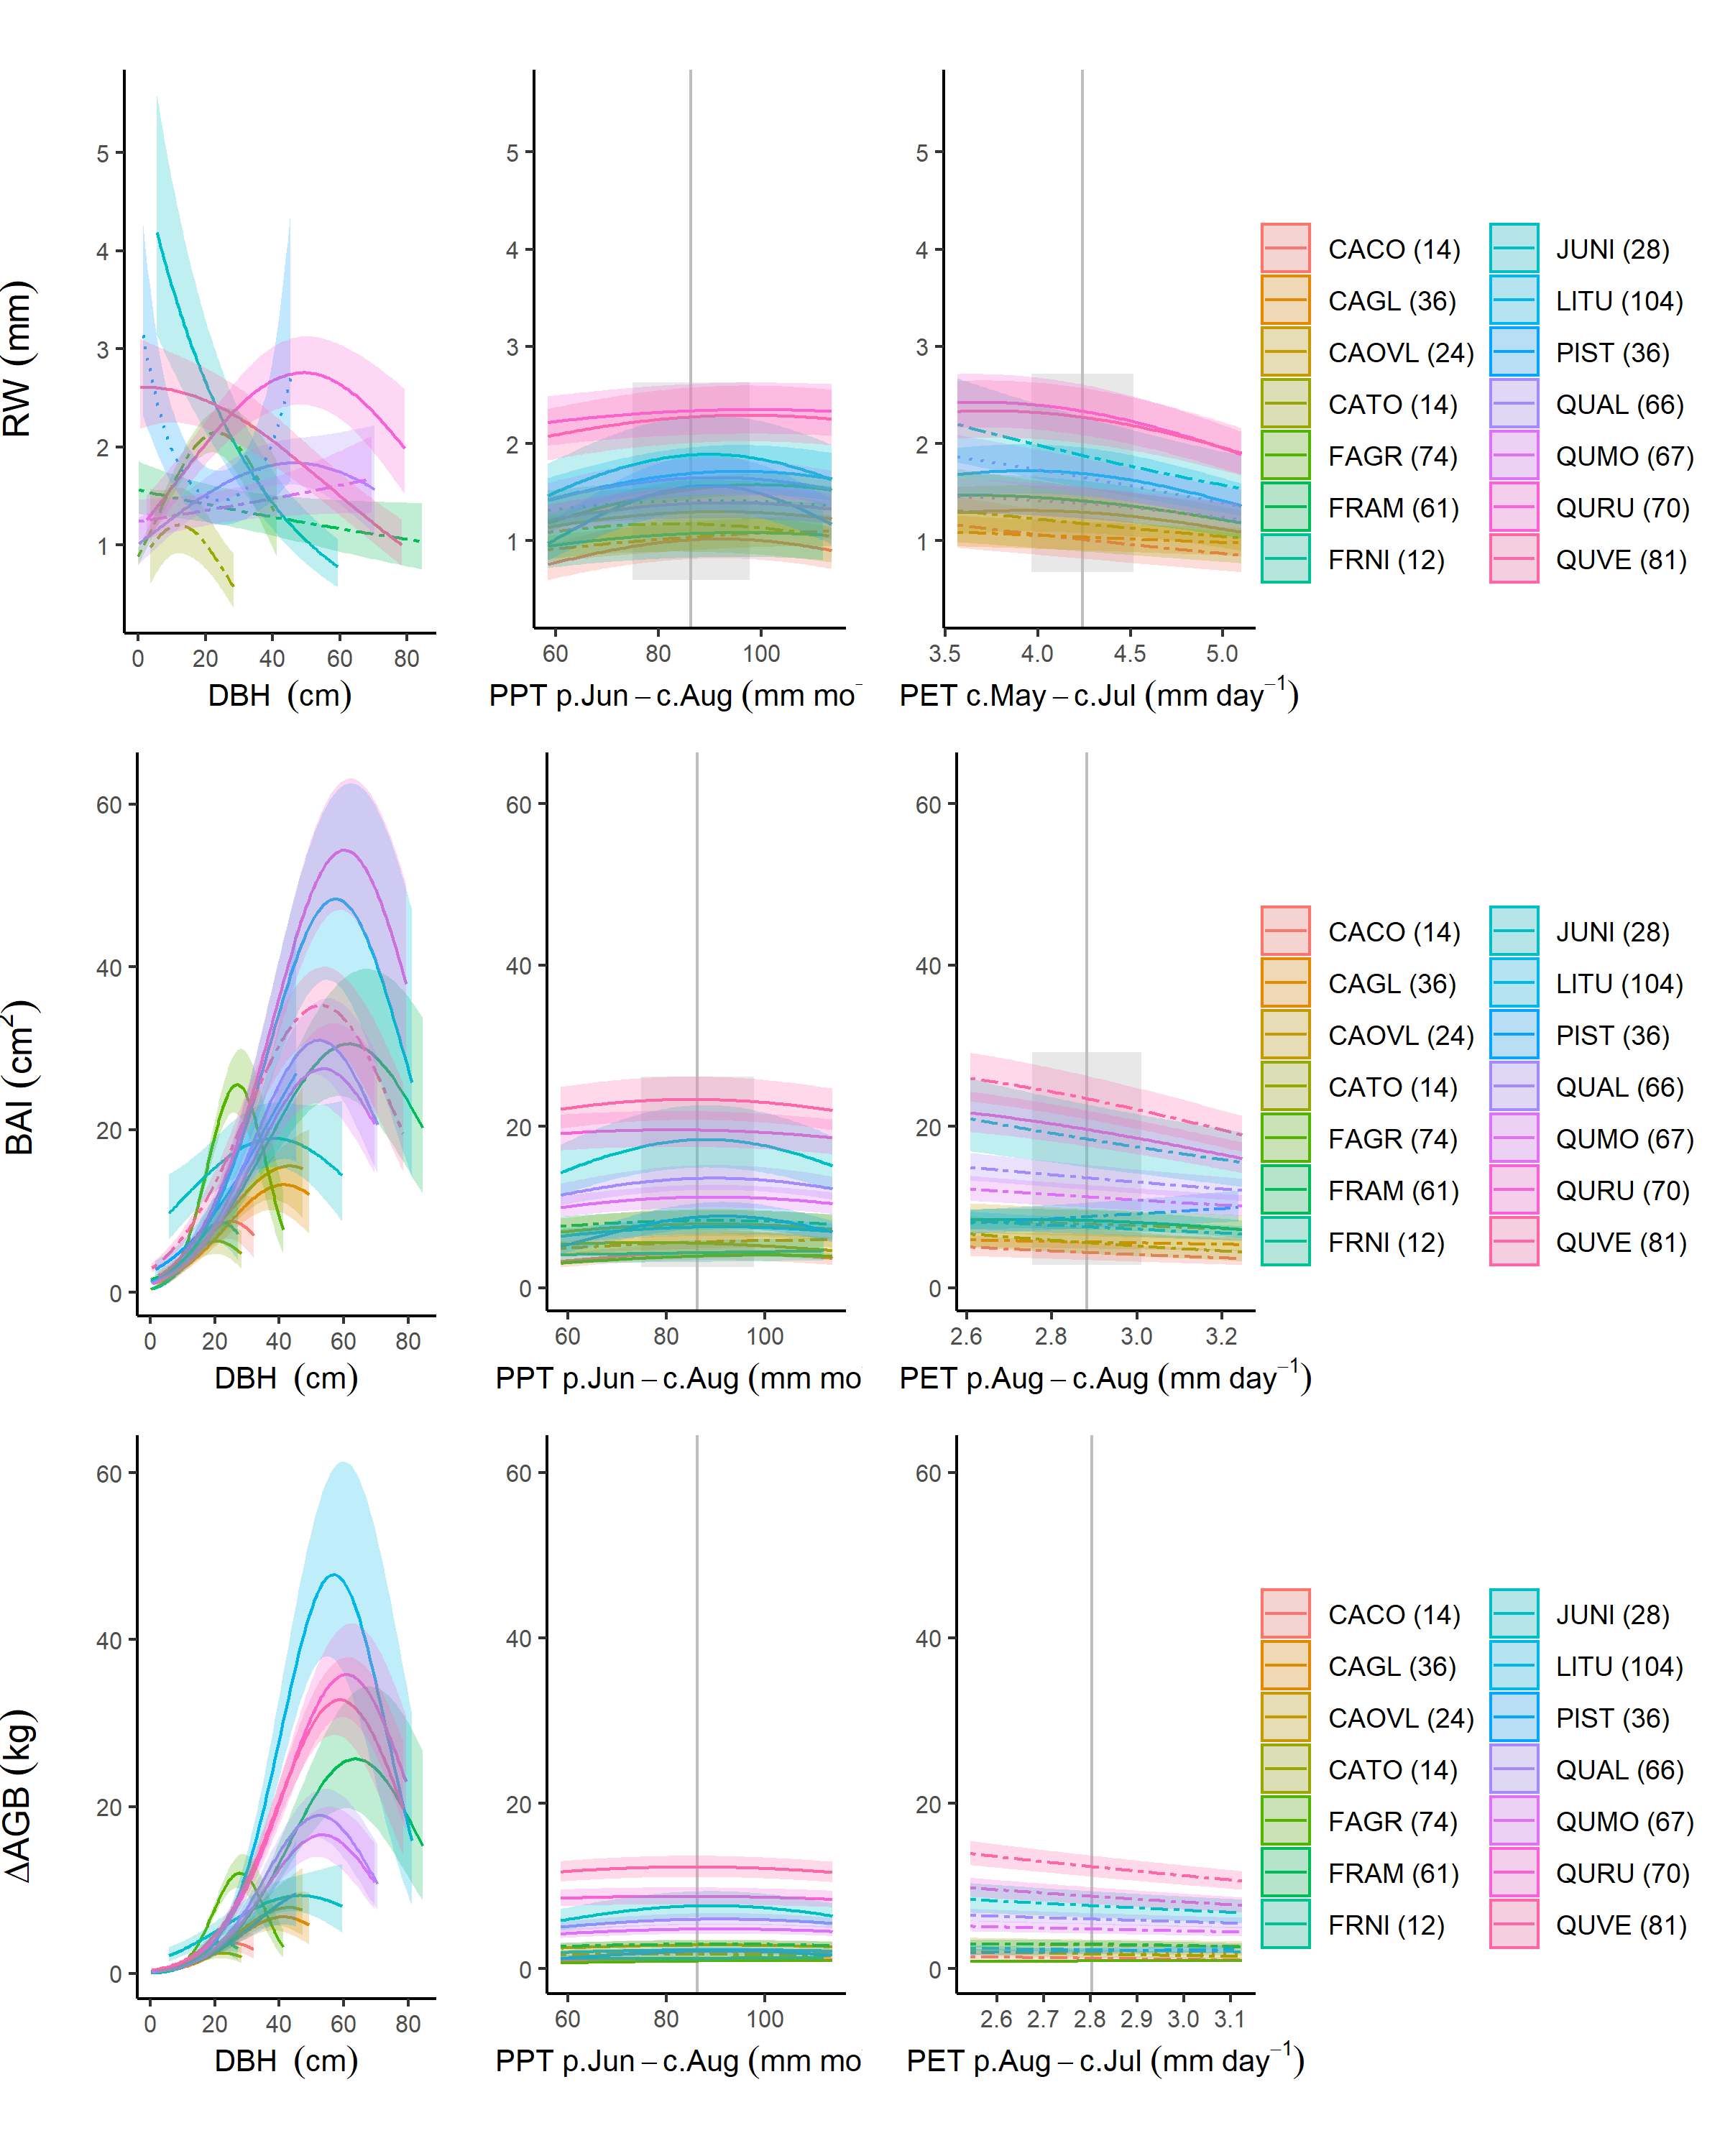
\includegraphics[width=0.75\textwidth,height=\textheight]{/Users/kteixeira/Dropbox (Smithsonian)/GitHub/EcoClimLab/ForestGEO-climate-sensitivity/results/composite_plots/SCBI.png}
\caption{\textbf{Figure S9 \textbar{} Best GLS models for SCBI
(Virginia, USA) for all three growth metrics: \(\Delta r\), \(BAI\), and
\(\Delta AGB\).} Precipitation and temperature group variables are as
selected by \emph{climwin} (p=previous year, c=current year). For each
species, relationships are plotted if included in top model, with
best-fit polynomials plotted with solid lines when both first- and
second-order terms are signficant, dashed lines when only one term is
signficant, and dotted lines when neither is signficant. Transparent
ribbons indicate 95\% confidence intervals. Vertical grey lines indicate
the long-term mean for the climate variable, shading indicates 1 SD.}
\end{figure}

\newpage

\hypertarget{figure-s10.-best-gls-models-for-lilly-dickey-woods-indiana-usa}{%
\subsection{Figure S10. Best GLS models for Lilly Dickey Woods (Indiana,
USA)}\label{figure-s10.-best-gls-models-for-lilly-dickey-woods-indiana-usa}}

\begin{figure}
\centering
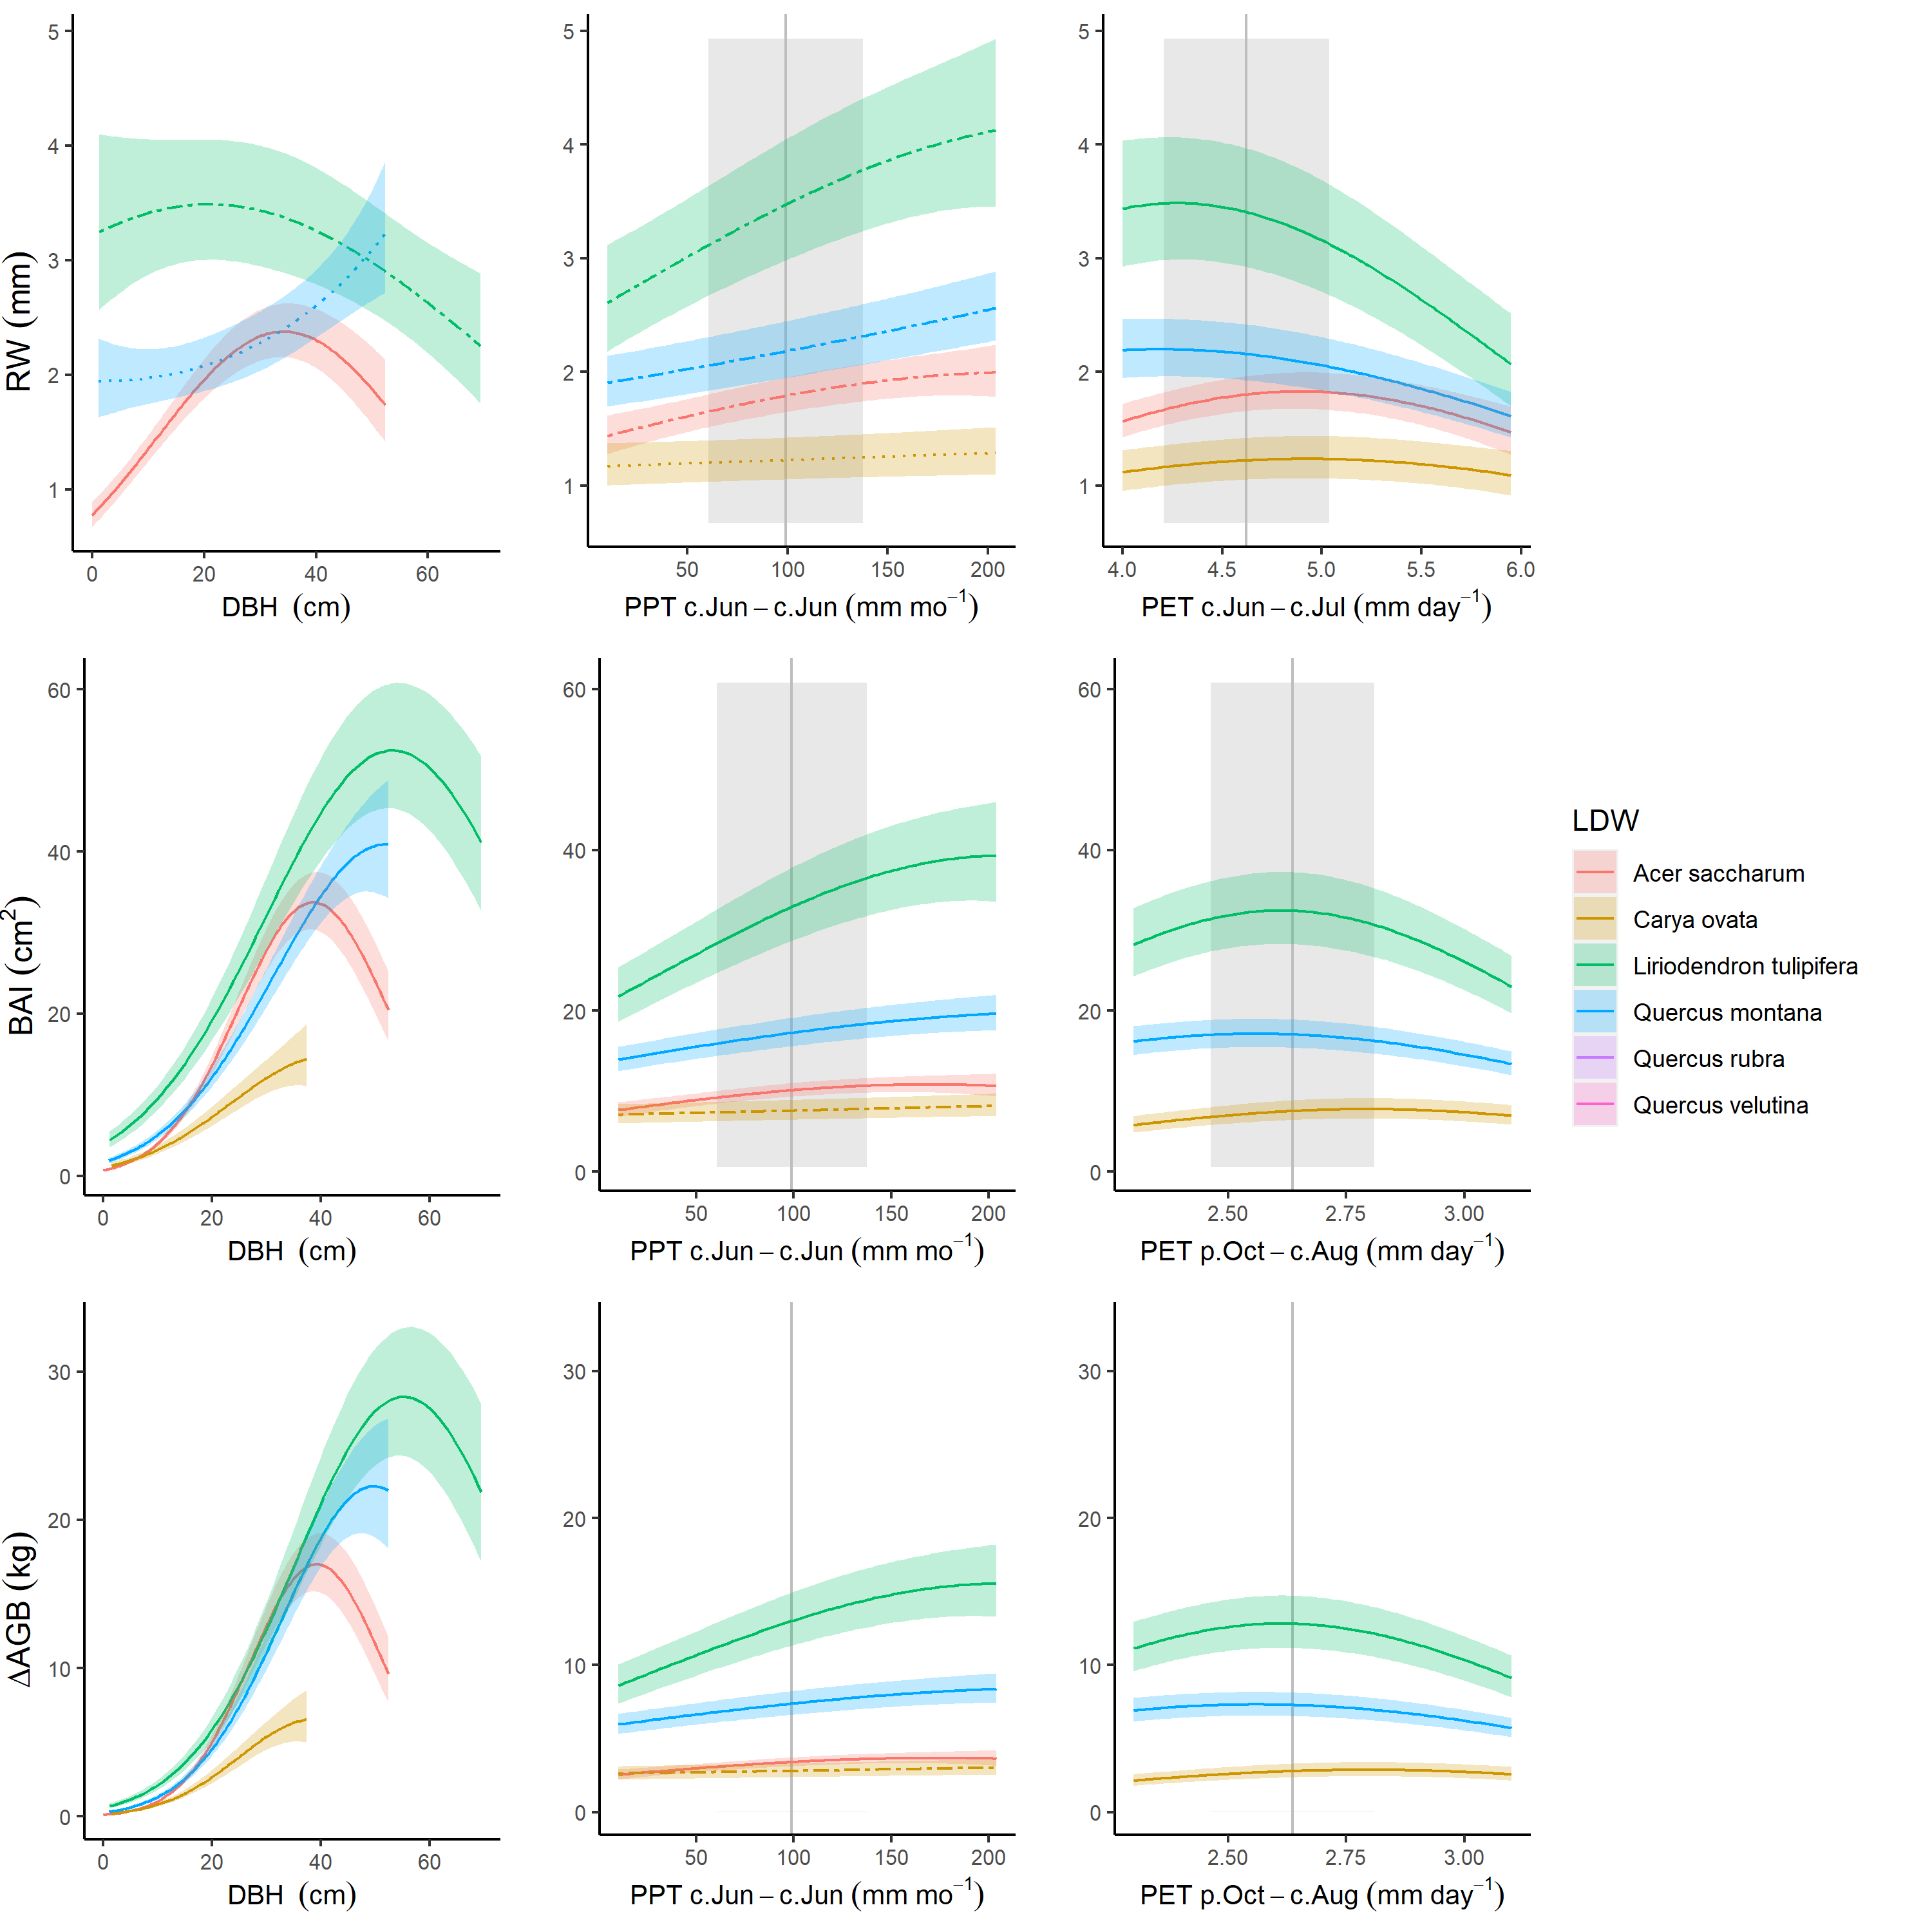
\includegraphics[width=0.75\textwidth,height=\textheight]{/Users/kteixeira/Dropbox (Smithsonian)/GitHub/EcoClimLab/ForestGEO-climate-sensitivity/results/composite_plots/LillyDickey.png}
\caption{\textbf{Figure S10 \textbar{} Best GLS models for Lilly Dickey
Woods (Indiana, USA) for all three growth metrics: \(\Delta r\),
\(BAI\), and \(\Delta AGB\).} Precipitation and temperature group
variables are as selected by \emph{climwin} (p=previous year, c=current
year). For each species, relationships are plotted if included in top
model, with best-fit polynomials plotted with solid lines when both
first- and second-order terms are signficant, dashed lines when only one
term is signficant, and dotted lines when neither is signficant.
Transparent ribbons indicate 95\% confidence intervals. Vertical grey
lines indicate the long-term mean for the climate variable, shading
indicates 1 SD.}
\end{figure}

\newpage

\hypertarget{figure-s11.-best-gls-models-for-harvard-forest-massachusetts-usa}{%
\subsection{Figure S11. Best GLS models for Harvard Forest
(Massachusetts,
USA)}\label{figure-s11.-best-gls-models-for-harvard-forest-massachusetts-usa}}

\begin{figure}
\centering
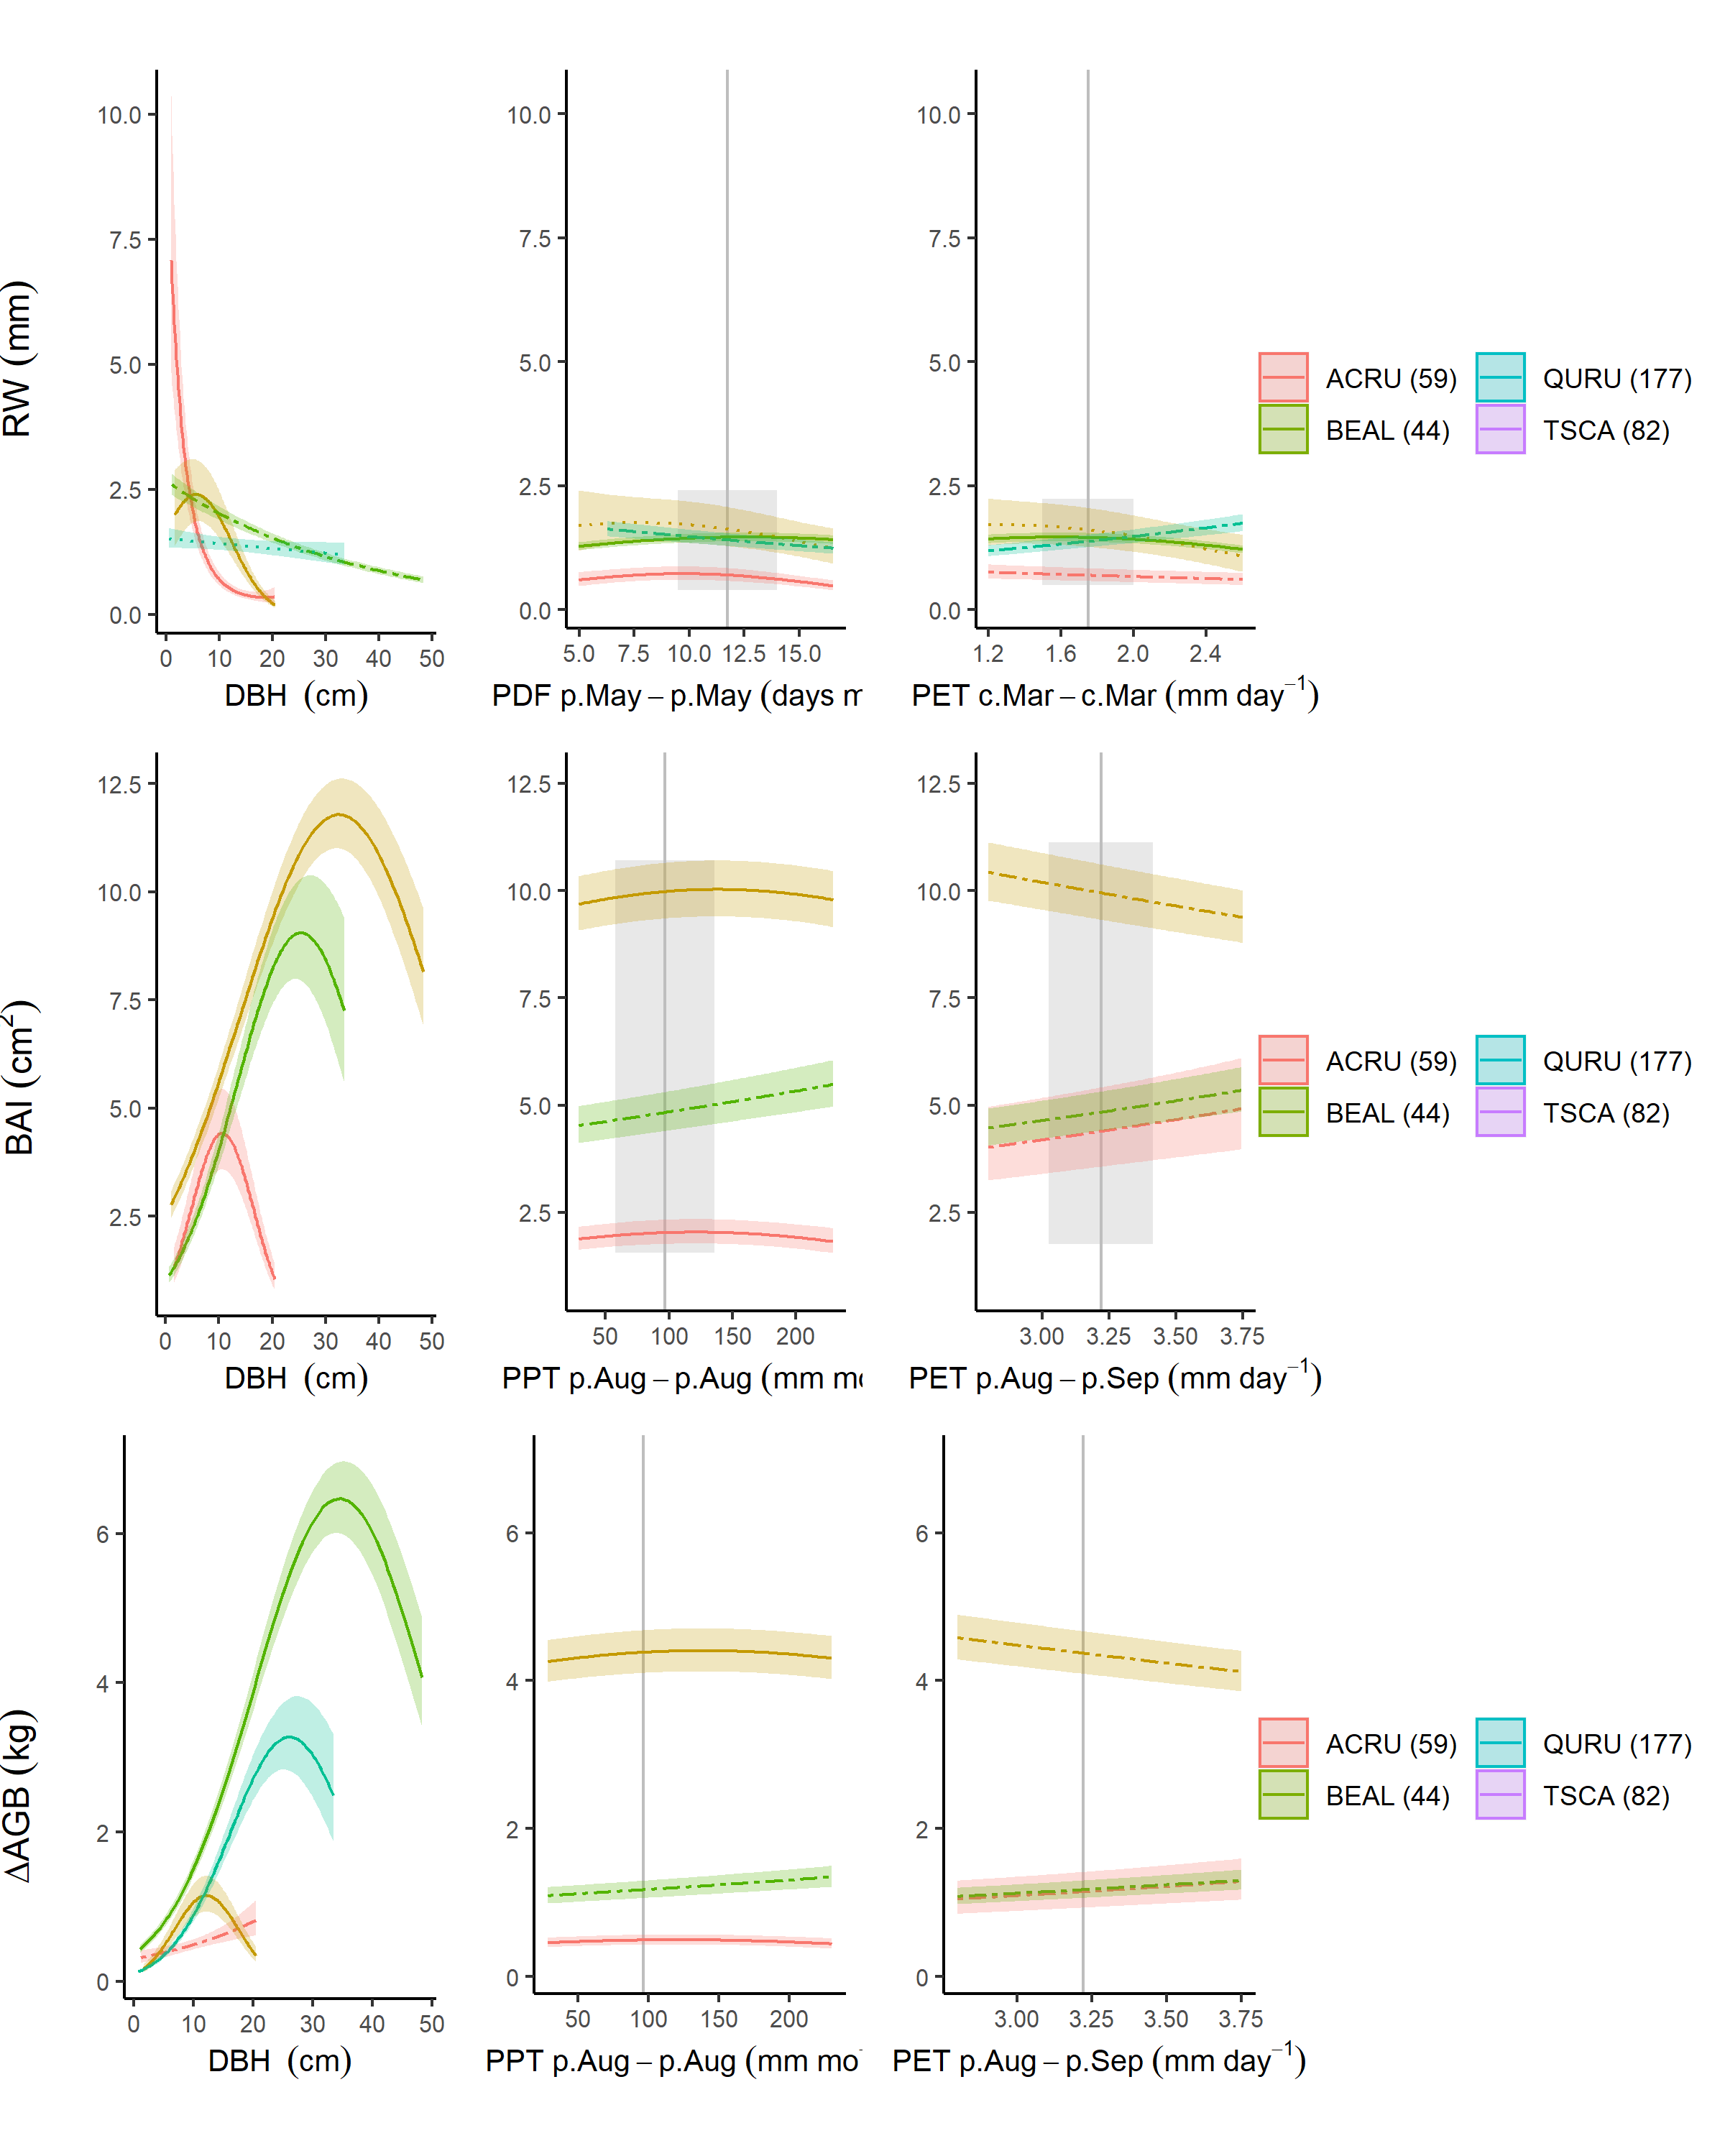
\includegraphics[width=0.75\textwidth,height=\textheight]{/Users/kteixeira/Dropbox (Smithsonian)/GitHub/EcoClimLab/ForestGEO-climate-sensitivity/results/composite_plots/HarvardForest.png}
\caption{\textbf{Figure S11 \textbar{} Best GLS models for Harvard
Forest (Massachusetts, USA) for all three growth metrics: \(\Delta r\),
\(BAI\), and \(\Delta AGB\).} Precipitation and temperature group
variables are as selected by \emph{climwin} (p=previous year, c=current
year). For each species, relationships are plotted if included in top
model, with best-fit polynomials plotted with solid lines when both
first- and second-order terms are signficant, dashed lines when only one
term is signficant, and dotted lines when neither is signficant.
Transparent ribbons indicate 95\% confidence intervals. Vertical grey
lines indicate the long-term mean for the climate variable, shading
indicates 1 SD.}
\end{figure}

\newpage

\hypertarget{figure-s12.-best-gls-models-for-niobrara-hansley-nebraska-usa}{%
\subsection{Figure S12. Best GLS models for Niobrara/ Hansley (Nebraska,
USA)}\label{figure-s12.-best-gls-models-for-niobrara-hansley-nebraska-usa}}

\newpage

\hypertarget{figure-s13.-best-gls-models-for-zofin-czech-republic}{%
\subsection{Figure S13. Best GLS models for Zofin (Czech
Republic)}\label{figure-s13.-best-gls-models-for-zofin-czech-republic}}

\begin{figure}
\centering
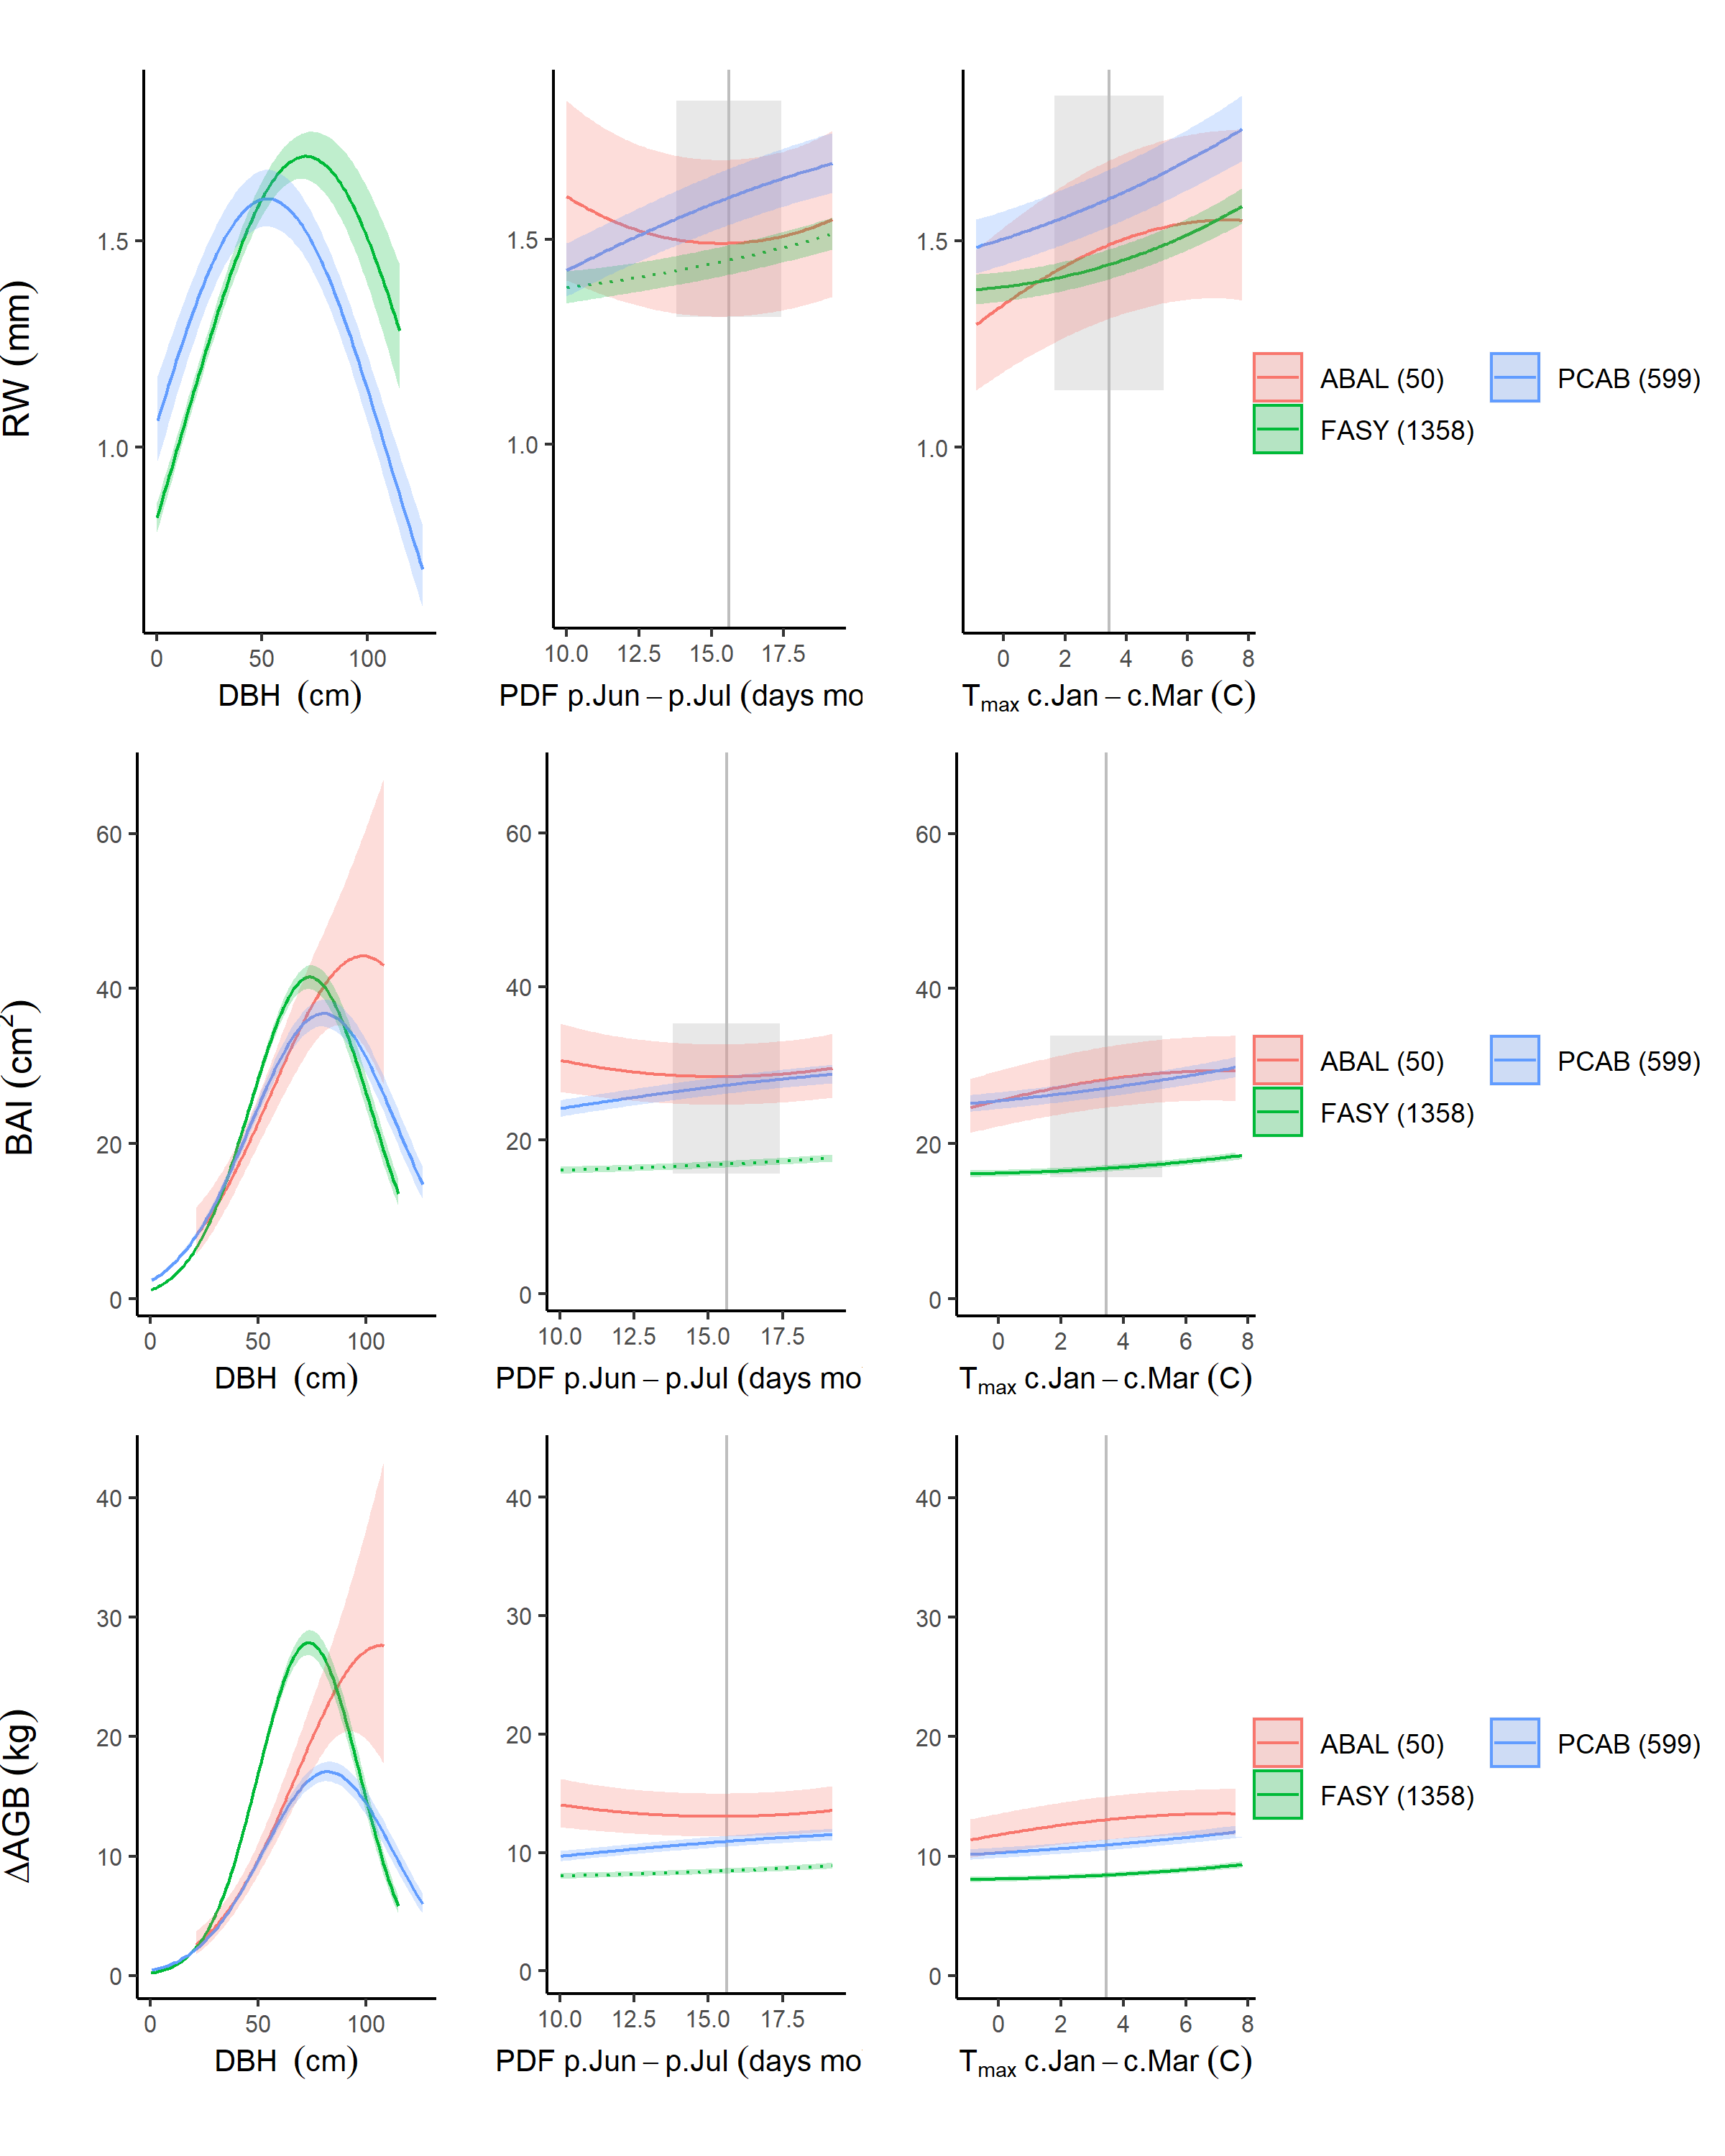
\includegraphics[width=0.75\textwidth,height=\textheight]{/Users/kteixeira/Dropbox (Smithsonian)/GitHub/EcoClimLab/ForestGEO-climate-sensitivity/results/composite_plots/Zofin.png}
\caption{\textbf{Figure S13 \textbar{} Best GLS models for Zofin (Czech
Republic) for all three growth metrics: \(\Delta r\), \(BAI\), and
\(\Delta AGB\).} Precipitation and temperature group variables are as
selected by \emph{climwin} (p=previous year, c=current year). For each
species, relationships are plotted if included in top model, with
best-fit polynomials plotted with solid lines when both first- and
second-order terms are signficant, dashed lines when only one term is
signficant, and dotted lines when neither is signficant. Transparent
ribbons indicate 95\% confidence intervals. Vertical grey lines indicate
the long-term mean for the climate variable, shading indicates 1 SD.}
\end{figure}

\newpage

\hypertarget{figure-s14.-best-gls-models-for-scotty-creek-nw-territories-canada}{%
\subsection{Figure S14. Best GLS models for Scotty Creek (NW
Territories,
Canada)}\label{figure-s14.-best-gls-models-for-scotty-creek-nw-territories-canada}}

\begin{figure}
\centering
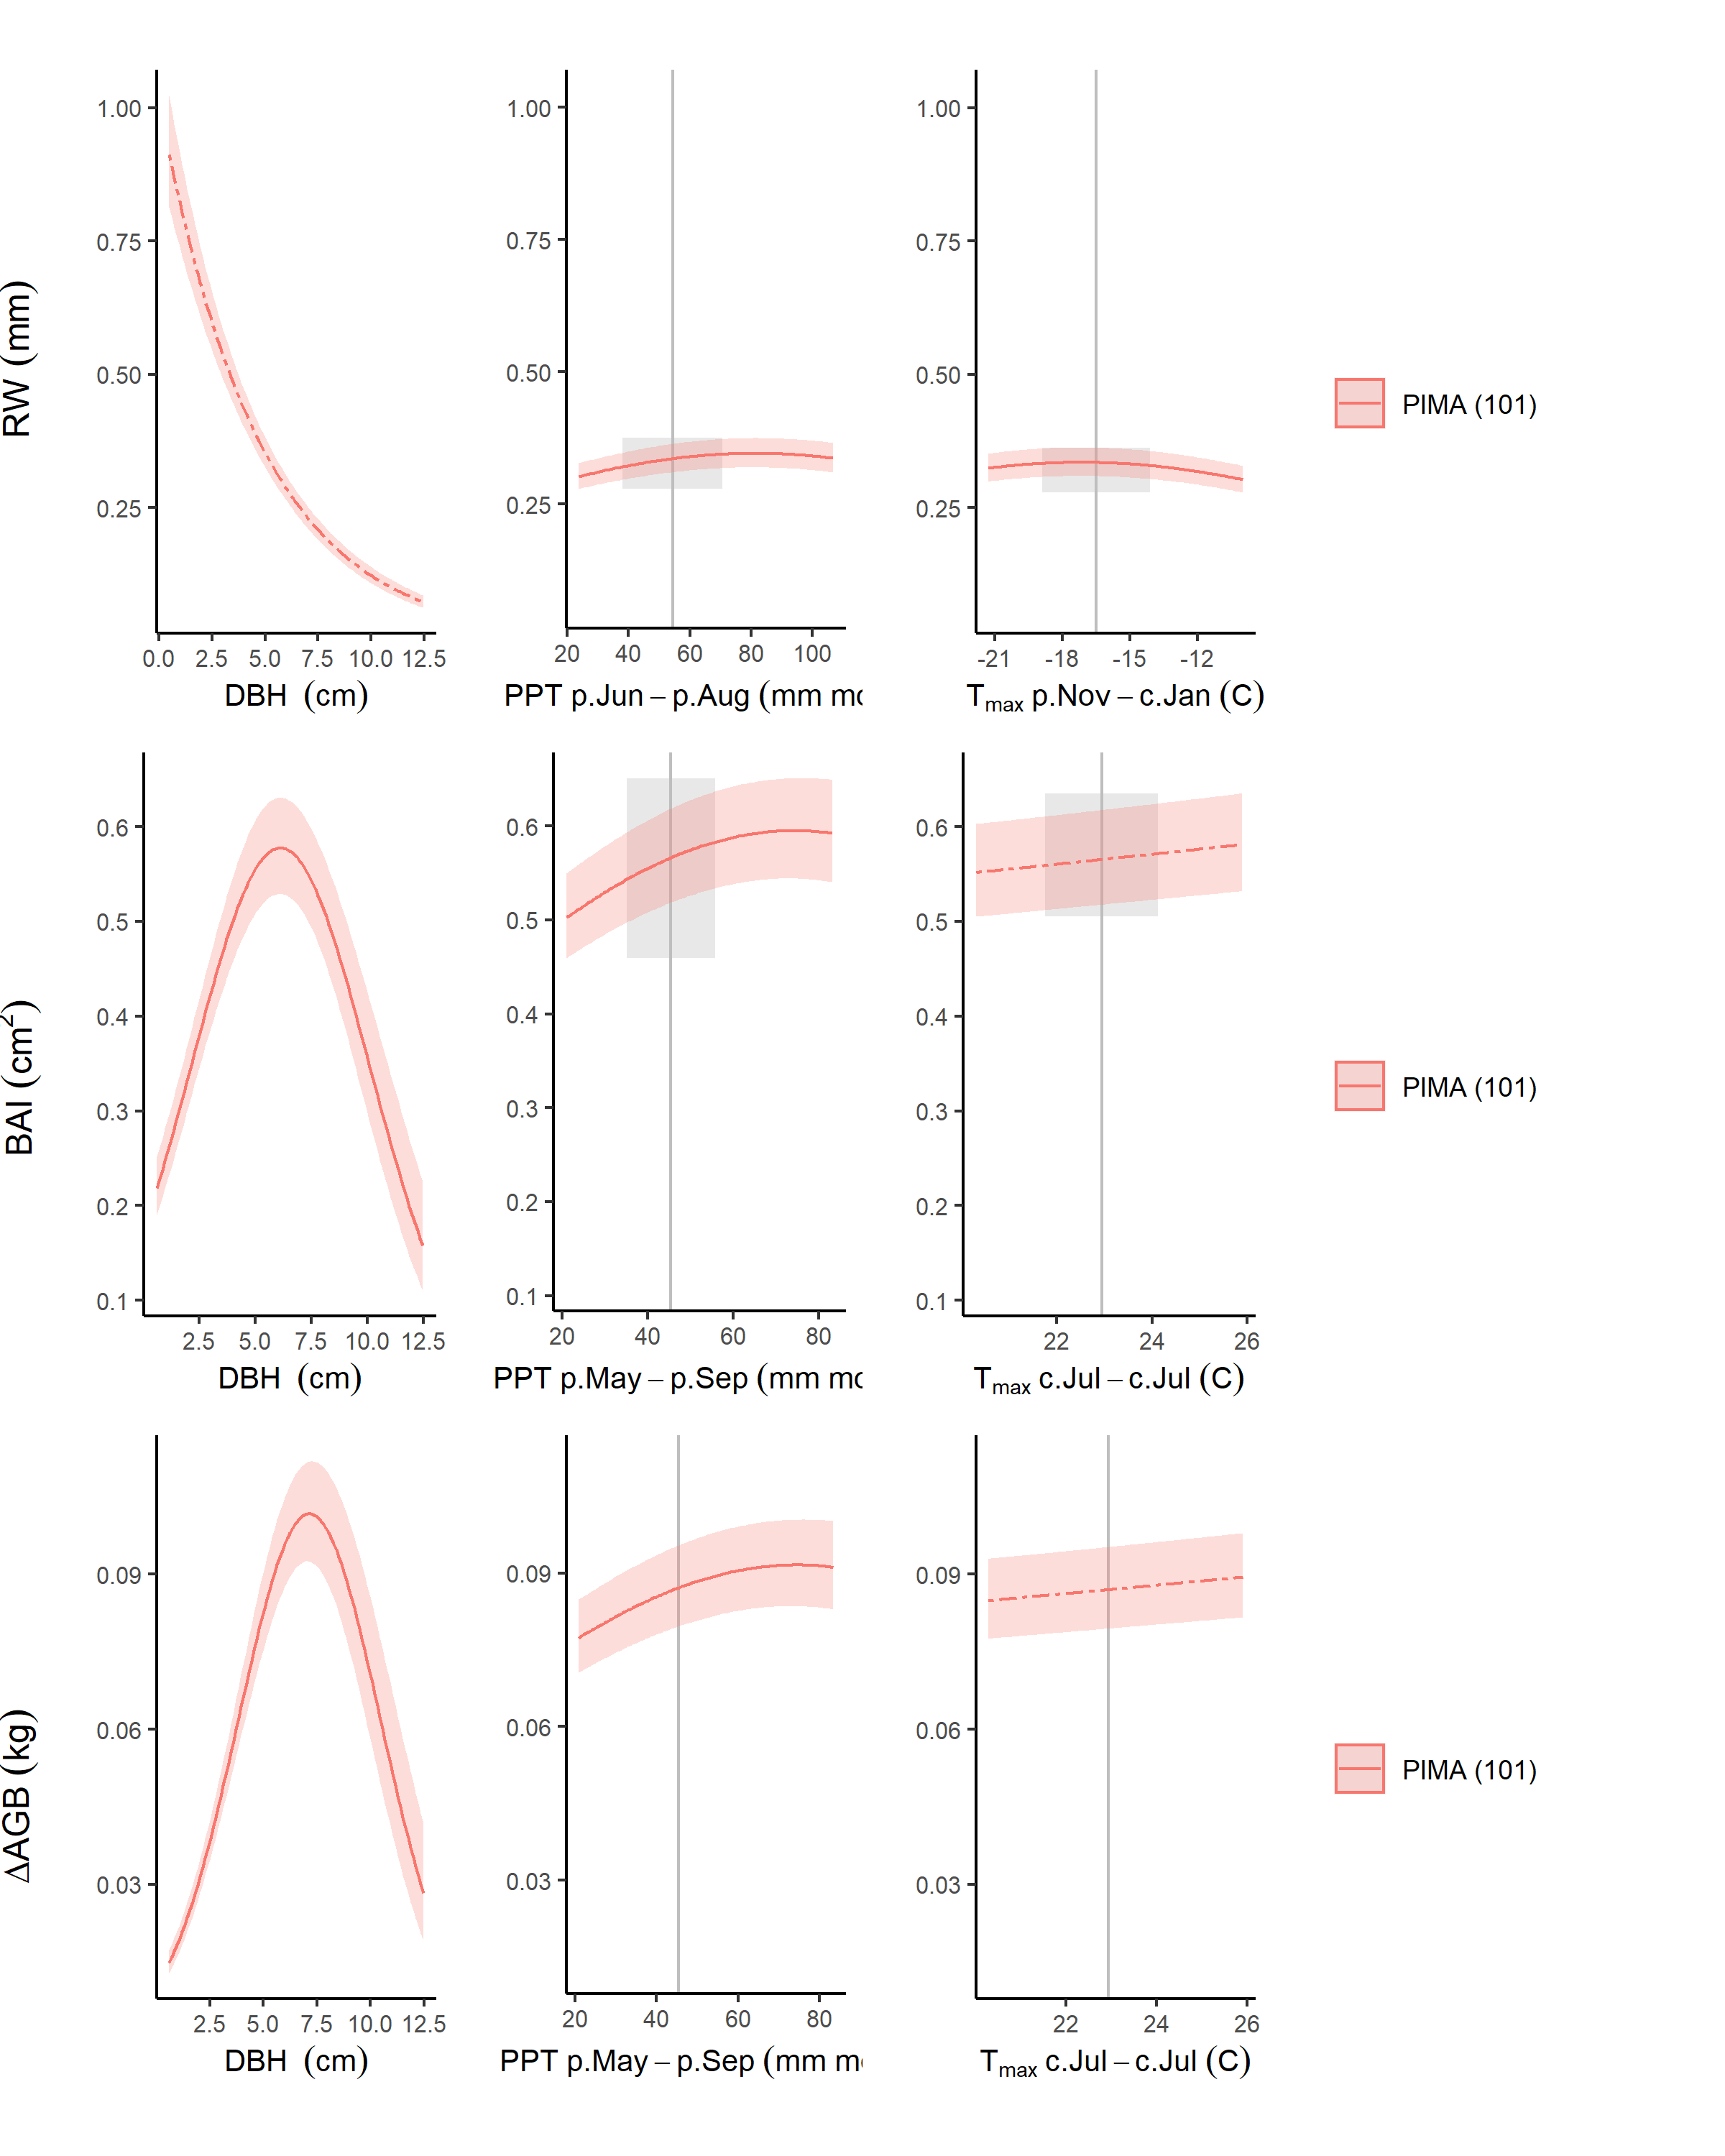
\includegraphics[width=0.75\textwidth,height=\textheight]{/Users/kteixeira/Dropbox (Smithsonian)/GitHub/EcoClimLab/ForestGEO-climate-sensitivity/results/composite_plots/ScottyCreek.png}
\caption{\textbf{Figure S14 \textbar{} Best GLS models for Scotty Creek
(NW Territories, Canada) for all three growth metrics: \(\Delta r\),
\(BAI\), and \(\Delta AGB\).} Precipitation and temperature group
variables are as selected by \emph{climwin} (p=previous year, c=current
year). For each species, relationships are plotted if included in top
model, with best-fit polynomials plotted with solid lines when both
first- and second-order terms are signficant, dashed lines when only one
term is signficant, and dotted lines when neither is signficant.
Transparent ribbons indicate 95\% confidence intervals. Vertical grey
lines indicate the long-term mean for the climate variable, shading
indicates 1 SD.}
\end{figure}

\newpage

\hypertarget{si-references}{%
\subsection*{SI References}\label{si-references}}
\addcontentsline{toc}{subsection}{SI References}

\hypertarget{refs}{}
\begin{cslreferences}
\leavevmode\hypertarget{ref-aus_de_ar_tree_2018}{}%
Aus de Ar, R. (2018). Tree Rings of Pinus ponderosa and Juniperus
virginiana Show Different Responses to Stand Density and Water
Availability in the Nebraska Grasslands. \emph{The American Midland
Naturalist}, \emph{180}(1), 18.
doi:\href{https://doi.org/10.1674/0003-0031-180.1.18}{10.1674/0003-0031-180.1.18}

\leavevmode\hypertarget{ref-bumann_assessing_2019}{}%
Bumann, E., Awada, T., Wardlow, B., Hayes, M., Okalebo, J., Helzer, C.,
\ldots{} Cherubini, P. (2019). Assessing responses of \emph{Betula}
\emph{Papyrifera} to climate variability in a remnant population along
the Niobrara River Valley in Nebraska, U.S.A., Through dendroecological
and remote-sensing techniques. \emph{Canadian Journal of Forest
Research}, \emph{49}(5), 423--433.
doi:\href{https://doi.org/10.1139/cjfr-2018-0206}{10.1139/cjfr-2018-0206}

\leavevmode\hypertarget{ref-helcoski_growing_2019}{}%
Helcoski, R., Tepley, A. J., Pederson, N., McGarvey, J. C., Meakem, V.,
Herrmann, V., \ldots{} Anderson-Teixeira, K. J. (2019). Growing season
moisture drives interannual variation in woody productivity of a
temperate deciduous forest. \emph{New Phytologist}, \emph{223}(3),
1204--1216.
doi:\href{https://doi.org/10.1111/nph.15906}{10.1111/nph.15906}

\leavevmode\hypertarget{ref-kaspar_species-specific_nodate}{}%
Kašpar, K., Tumajer, J., Vašíčková, I., \& Šamonil, P. (n.d.).
Species-specific climate-growth interactions determine the future tree
species dynamics of the mixed Central European mountain forests.

\leavevmode\hypertarget{ref-maxwell_declining_2016}{}%
Maxwell, J. T., Harley, G. L., \& Robeson, S. M. (2016). On the
declining relationship between tree growth and climate in the Midwest
United States: The fading drought signal. \emph{Climatic Change},
\emph{138}(1-2), 127--142.
doi:\href{https://doi.org/10.1007/s10584-016-1720-3}{10.1007/s10584-016-1720-3}

\leavevmode\hypertarget{ref-sniderhan_growth_2016}{}%
Sniderhan, A. E., \& Baltzer, J. L. (2016). Growth dynamics of black
spruce ( \emph{Picea} \emph{Mariana} ) in a rapidly thawing
discontinuous permafrost peatland: Growth Dynamics Boreal Peatlands.
\emph{Journal of Geophysical Research: Biogeosciences}, \emph{121}(12),
2988--3000.
doi:\href{https://doi.org/10.1002/2016JG003528}{10.1002/2016JG003528}

\leavevmode\hypertarget{ref-tumajer_increasing_2017}{}%
Tumajer, J., Altman, J., Štěpánek, P., Treml, V., Doležal, J., \&
Cienciala, E. (2017). Increasing moisture limitation of Norway spruce in
Central Europe revealed by forward modelling of tree growth in tree-ring
network. \emph{Agricultural and Forest Meteorology}, \emph{247}, 56--64.
doi:\href{https://doi.org/10.1016/j.agrformet.2017.07.015}{10.1016/j.agrformet.2017.07.015}

\leavevmode\hypertarget{ref-vlam_temperature_2014}{}%
Vlam, M., Baker, P. J., Bunyavejchewin, S., \& Zuidema, P. A. (2014).
Temperature and rainfall strongly drive temporal growth variation in
Asian tropical forest trees. \emph{Oecologia}, \emph{174}(4),
1449--1461.
doi:\href{https://doi.org/10.1007/s00442-013-2846-x}{10.1007/s00442-013-2846-x}
\end{cslreferences}

\end{document}
